\documentclass{article}
\usepackage[utf8]{inputenc}
\usepackage[T1]{fontenc} % Output font encoding for international characters
\usepackage{graphicx} % Required for including images
\usepackage{booktabs} % Required for better horizontal rules in tables
\usepackage{listings} % Required for insertion of code
\usepackage{enumerate} % To modify the enumerate environment
\usepackage{hyperref}
\usepackage{subcaption} % for captions for multiple images per figure



\title{	
	\normalfont\normalsize
	\textsc{National Technical University of Athens}\\ % Your university, school and/or department name(s)
	\vspace{25pt} % Whitespace
	\rule{\linewidth}{0.5pt}\\ % Thin top horizontal rule
	\vspace{20pt} % Whitespace
	{\LARGE Creating an elevation map of a staircase using 
Intel RealSense and ROS}\\ % The assignment title
	\vspace{12pt} % Whitespace
	\rule{\linewidth}{2pt}\\ % Thick bottom horizontal rule
	\vspace{12pt} % Whitespace
}
\author{\LARGE Zarras Ioannis} % Your name
\medskip
\date{Department of Mechanical Engineering --- \today}

\begin{document}
\maketitle
\tableofcontents


\section{Overview}

The goal of this project is to review software packages developed for elevation mapping. Most algorithms require odometry data, as well as depth and color images captured in real time to produce an elevation map. The hardware used in this project to provide these measurements consists of the Intel® RealSense™ Tracking Camera T265 \href{https://www.intelrealsense.com/tracking-camera-t265/}{[1]} and the  Intel® RealSense™ Depth Camera D435i \href{https://www.intelrealsense.com/depth-camera-d435i/}{[2]}. The packages reviewed were configured to use data from these two sensors. The Realsense cameras were also reviewed and compared with similar commercially available cameras.

\section{Theoretical framework}

Standard digital cameras output images as a 2D grid of pixels. Each pixel has values associated with it – usually we think of those as Red, Green and Blue, or RGB. Each attribute has a number from 0 to 255, so black, for example, is (0,0,0) and a pure bright red would be (255,0,0). Thousands to millions of pixels together create the kind of photographs we are all very familiar with. A depth camera on the other hand, has pixels which have a different numerical value associated with them, that number being the distance from the camera, or “depth.” Some depth cameras have both an RGB and a depth system, which can give pixels with all four values, or RGB-D.\href{https://www.intelrealsense.com/beginners-guide-to-depth/}{[3]} Constructing a 3D map utilizing a depth camera mounted on a moving base poses the challenge of organizing each newly captured RGB-D frame in 3D space. Namely, finding its position and orientation relative to the previously captured frame so that the map is constructed piece by piece, like a three-dimensional puzzle. To accurately determine the position and orientation of each RGB-D frame, information about the location and orientation of the camera at the moment of capturing each frame is required.

Simultaneous localization and mapping (SLAM) is the computational problem of constructing or updating a map of an unknown environment while simultaneously keeping track of an agent's location within it. While this initially appears to be a chicken-and-egg problem there are several algorithms known for solving it, at least approximately, in tractable time for certain environments.\href{https://en.wikipedia.org/wiki/Simultaneous_localization_and_mapping}{[4]}
To construct our elevation map, we will be implementing SLAM using depth data from the D435i sensor and odometry data from the T265 sensor.

\section{Technological framework}

\subsection{Depth Sensing}

The two most prominent technologies that are commonly utilized for capturing depth are lidar sensors and depth camera sensors. The pros and cons of each of those technologies will be briefly discussed:

\subsubsection{Principle}

Lidar: It is an acronym of "light detection and ranging", also called 3-D laser scanning. It is a method for determining ranges (variable distance) by targeting an object with a laser and measuring the time for the reflected light to return to the receiver \href{https://en.wikipedia.org/wiki/Lidar}{[5]}. \\
Depth Camera: It either:

\begin{itemize}

\item Measures the depth of the target object by illuminating the object with controlled patterns of dots using infra-red light or LED and analyzing the reflected light pattern
\item Uses stereo triangulation to determine the depth of an object, much like a human brain uses the stereoscopic view from our eyes\href{https://lidarradar.com/info/differences-between-the-lidar-systems-and-depth-camera}{[6]}.
\item Combine the above two methods.
\item There are also Time of Flight Depth Cameras, which similarily to Lidar, illuminate the scene with a controlled laser or LED source and then analyze the wavelength of the reflected light as well as the time for it to return to the receiver\href{https://www.researchgate.net/publication/347124772_An_Overview_of_Depth_Cameras_and_Range_Scanners_Based_on_Time-of-Flight_Technologies}{[7]}.

\end{itemize}

\subsubsection{Cost}

Lidar: High-resolution Lidar system is considered to be very expensive compared to depth camera hardware. For reference, google's Waymo autonomous vehicle requires three lidar sensors costing 7,000\$ each while Tesla’s Model 3, with \$10,000 full-self driving (FSD) add-on, already has all the necessary computer hardware and sensors for autonomous driving, utilizing cameras, ultrasonic and radar sensors\href{https://www.voltequity.com/article/why-lidar-is-doomed}{[8]}.

Depth Camera: Cameras are inexpensive with cost-effective hardware and high-resolution image sensors. Even low-cost commercial lenses can be used to capture high quality footage and produce high quality depth streams.
 
\subsubsection{Weaknesses}

Lidar: The laser sensors are susceptible to bad weather conditions. They are unable to capture shades or color details of detected objects.

Depth Camera: They are susceptible to unique noise such as range ambiguity, when reflected pulses of light interfere with emmited pulses, scattering, and motion blur. Range ambiguity noise and scattering noise are unique to time of flight depth cameras. The measured depth accuracy drops significantly as the distance from the measured object increases. This is true for both time of flight and stereo depth cameras. 

\begin{figure}[h] % [h] forces the figure to be output where it is defined in the code (it suppresses floating)
	\centering
	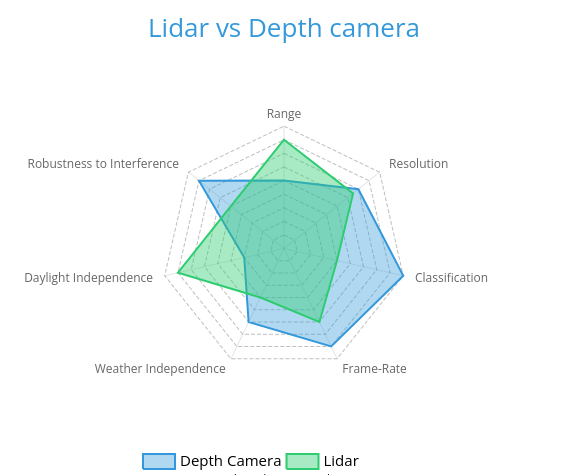
\includegraphics[width=1\columnwidth]{report1-img023.png} % Example image
	\caption{A radar chart displaying observations on lidar and depth camera pros and cons.}
\end{figure}

Ultimately, depth cameras are a good tradeoff between performance and cost and were thus chosen for this project.


\subsection{Localization}

It is quite common to acquire the information needed for localization by wheel encoders (wheeled odometry) or an accurate IMU fixed on the robot. IMUs have high variance and can be noisy, while there are a number of error sources in wheel odometry methods, the most significant being wheel slippage in uneven terrain or slippery floors.

However, it is also possible to track a robot's motion solely by processing visual data. This process is known as visual odometry. It is achieved by utilizing image processing algorithms to translate the visual difference between two consecutive frames to actual translation and rotation of the observer that captured them. For example, let there be two consecutively captured frames, say $frame_1$ and $frame_2$, where $frame_2$ has been captured slightly after $frame_1$. If a correspondence of points or features between these frames is made and it is deducted that most of the objects on $frame_2$ are now seen as though they have moved (transposed) slightly to the right when compared to $frame_1$, then we could assume that the robot that captured the frames was moving slightly to the left upon capturing $frame_2$. This is of course a simplification but most image processing algorithms follow the same principle \href{https://en.wikipedia.org/wiki/Correspondence_problem}{[9]}. Using visual odometry to build a 3D map is a procedure known as V-SLAM (Visual Simultaneous Localization and Mapping). 

Achieving V-SLAM in real time is a computationally intensive process. Although visual localization can be accomplished using the RGB-D images taken from the depth camera that is being used for mapping the environment, a camera with a wider field of view and a dedicated embedded system for V-SLAM algorithms will provide faster and more accurate results. As a result, a dedicated tracking camera was chosen for that purpose.

\section{Hardware}

To implement the elevation mapping the D435i Intel® RealSense™  Depth camera was used alongside the T265 Intel® RealSense™  Tracking Camera. Intel offers a wide selection of RealSense Depth cameras. Thus, to select the appropriate camera we consulted the realsense website\href{https://www.intelrealsense.com/#Products}{[10]}:

\clearpage

\begin{table}[h] % [h] forces the table to be output where it is defined in the code (it suppresses floating)
\noindent\makebox[\textwidth]{%
    \begin{tabular}{l l l l}
        		\toprule
        		\textbf{Product} & \textit{Environment} & \textit{Range} & \textit{Field of View}\\
        		\midrule
        		D415 & Indoor/Outdoor & 0.16m-10m & 65°±2°×40°±1°× 72°± 2°\\
        		D435i & Indoor/Outdoor & 0.1m-10m & 86°×57°(±3°) \\
        		D435 & Indoor/Outdoor & 0.1m-10m & 86°×57°(±3°)\\
        		D455 & Indoor/Outdoor & 0.4m-20m & 86°×57°(±3°)\\
        		L515 & Indoor & 0.25m-9m & 70° × 55° (±2°)\\
        		SR305 & Indoor & 0.2m-1.5m & 69°±3° × 54°±2°\\
        		T265 & Indoor/Outdoor & None & 163±5°\\
        		\bottomrule
    \end{tabular}
}

\end{table}


\begin{table}[h] % [h] forces the table to be output where it is defined in the code (it suppresses floating)
\noindent\makebox[\textwidth]{%
    \begin{tabular}{l l l}
        		\toprule
        		\textbf{Product} & \textit{RGB Field of View} & \textit{Special} \\
        		\midrule
        		D415 & 69.4°×42.5°×77°(±3°) & Small FOV, high depth resolution \\
        		D435i & 69.4°×42.5°×77°(±3°) & IMU embedded \\
        		D435 & 69.4°×42.5°×77°(±3°) & None \\
        		D455 & 86°×57°(±3°) & IMU, newest, double range \\
        		L515 & 70°±3 × 43°±2 & Precision, indoor, small \\
        		SR305 & 68° × 41.5° (±2°) & Strictly indoor. cheapest \\
        		T265 & None & Tracking Camera. Widest FOV \\
        		\bottomrule
    \end{tabular}
}

\caption{Comparison of available Realsense Cameras}
\end{table}

The following conclusions can be drawn:
\begin{itemize}
  \item The D435 and D455 cameras have a large Field Of View. However, they use the same RGB sensor as the D415 which has a narrower FOV. For most mapping applications, the depth frames are cropped to match the dimensions of the RGB frames and thus the larger depth FOV of the D435 and D455 cameras might not be fully utilized. It should be noted that a wider field of view could mean a lower depth resolution if the same depth sensor is used.
  \item The minimum distance for reliable Depth estimation for the D400 series is 0.3m instead of 0.1m which intel claims, according to \href{https://www.youtube.com/watch?v=mFLZkdH1yLE}{[11]}. However, considering the use case of a stairway mapping, the above distance will not be an issue.
  \item The combination of D435 with the T265 gives precise depth estimation to the point of achieving voumetric and shape estimation of objects. It is a reliable combination for implementing SLAM \href{https://www.intelrealsense.com/tracking-camera-t265/}{[1]}.
  \item SLAM can be achieved by solely using the D455 or the D435i cameras by utilizing the embedded IMUs that they include, but it must be given that the motion of the robot is slow and the field of interest is relatively narrow.
  \item There is a ROS wrapper for all the above devices which is actively supported by Intel  \href{https://github.com/IntelRealSense/realsense-ros}{[12]}.
\end{itemize}

The combination of D435i alongside the T265 camera was chosen, for both indoor and outdoor SLAM implementations.

\subsection{The D435i Depth Camera}

There is a variety of methods for calculating depth, all come with strengths and weaknesses. The D435i depth camera utilizes the two most prominent methods, i.e., structured light and stereo vision.

\subsubsection{Structured Light and Coded Light}                    

Structured light and coded light depth cameras are technologies that rely on projecting light (usually infrared light) from some kind of emitter onto the scene. The projected light is patterned, either visually or over time, or some combination of the two. Since the projected pattern is known, how the sensor in the camera sees the pattern in the scene provides the depth information \href{https://www.intelrealsense.com/beginners-guide-to-depth/}{[3]}. For example, as demonstrated in Figure 2, if the pattern is a series of stripes projected onto a ball, the stripes would deform and bend around the surface of the ball in a specific way.

If the ball moves closer to the emitter, the pattern would change too. Using the disparity between an expected image and the actual image viewed by the camera, distance from the camera can be calculated for every pixel. Because this technology relies on accurately seeing a projected pattern of light, coded and structured light cameras do best indoors at relatively short ranges (depending on the power of the light emitted from the camera). Another issue with systems like this is that they are vulnerable to noise in the environment from other cameras or devices emitting infrared light. Ideal uses for coded light cameras are things like gesture recognition or background segmentation (also known as virtual green screen).

\begin{figure}[h] % [h] forces the figure to be output where it is defined in the code (it suppresses floating)
	\centering
	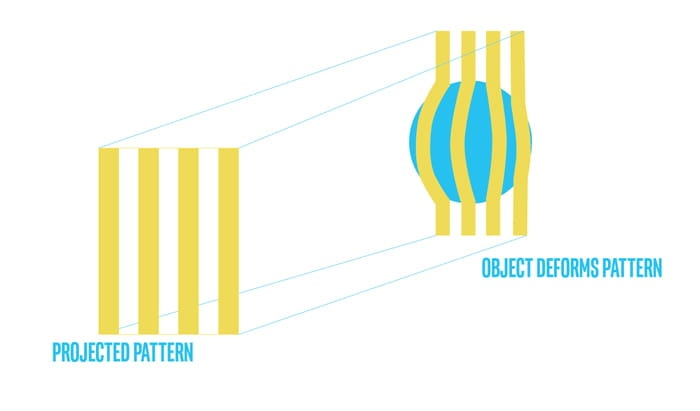
\includegraphics[width=1\columnwidth]{report1-img001.png} % Example image
	\caption{Deformation of structured light on a spherical object \href{https://www.intelrealsense.com/beginners-guide-to-depth/}{[3]}.}
\end{figure}

\subsubsection{Stereo Depth}

Stereo depth cameras also often project infrared light onto a scene to improve the accuracy of the data. However, unlike coded or structured light cameras, stereo cameras can use the whole spectrum of light to measure depth. For a stereo camera, infrared noise is just another source of light that illuminates the scene and can assist with depth measurements, even though it might interfere with the infrared light projection.

Stereo depth cameras have two sensors, spaced a small distance apart \href{https://www.intelrealsense.com/beginners-guide-to-depth/}{[3]}. A stereo camera takes the two images from these two sensors and compares them. Since the distance between the sensors is known, these comparisons give depth information. Stereo cameras work in a similar way to how we use our two eyes for depth perception. Our brains calculate the difference between the images that each eye receives. Objects closer to us will appear to move significantly from eye to eye image, where an object far away would appear to move very little.

Because stereo cameras use visual features to measure depth, they will work well in most lighting conditions including outdoors. The fact that the D435i camera of is equipped with an infrared projector means that in low lighting conditions, the camera can still perceive depth details. Another benefit of stereo depth cameras is that there are no limits to how many you can use in a particular space – the cameras don’t interfere with each other in the same way that a coded light or time of flight camera would.

The maximum distance these cameras can measure is directly related to how far apart the two image sensors are – the wider the baseline is, the further the camera can see. In fact, astronomers use a very similar technique to measure the distance of faraway stars, by measuring the position of a star in the sky at one point in time, and then measuring that same star six months later when the earth is at the furthest point in its orbit from the original measuring point. In this way, they can calculate the distance (or depth of the star) using a baseline of around 300 million kilometers \href{https://courses.lumenlearning.com/astronomy/chapter/surveying-the-stars/}{[13]}.

\begin{figure}[h] % [h] forces the figure to be output where it is defined in the code (it suppresses floating)
	\centering
	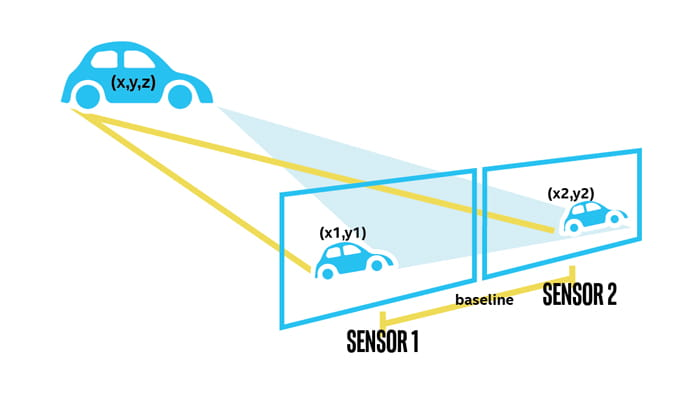
\includegraphics[width=1\columnwidth]{report1-img002.png} % Example image
	\caption{Representation of stereo depth vision \href{https://www.intelrealsense.com/beginners-guide-to-depth/}{[3]}.}
\end{figure}


\subsection{The T265 tracking camera}

Until recent years sailors would navigate by the stars, using their movements and positions to successfully find their way across oceans. The T265 tracking camera uses a combination of cameras and Inertial Measurement Units (IMU) to navigate in a similar way, performing V-SLAM by using visual features in the environment to track it’s way around even unknown spaces with accuracy. 

The Intel RealSense T265 Tracking Camera includes two fisheye lenses. A fisheye lens is an ultra wide-angle lens intended to create a wide panoramic or hemispherical image. Fisheye lenses can achieve an extremely wide field of view. Instead of producing images with straight lines of perspective (rectilinear images), fisheye lenses use a special mapping, which gives images a characteristic convex non-rectilinear appearance. 


\begin{figure}[h] % [h] forces the figure to be output where it is defined in the code (it suppresses floating)
	\centering
	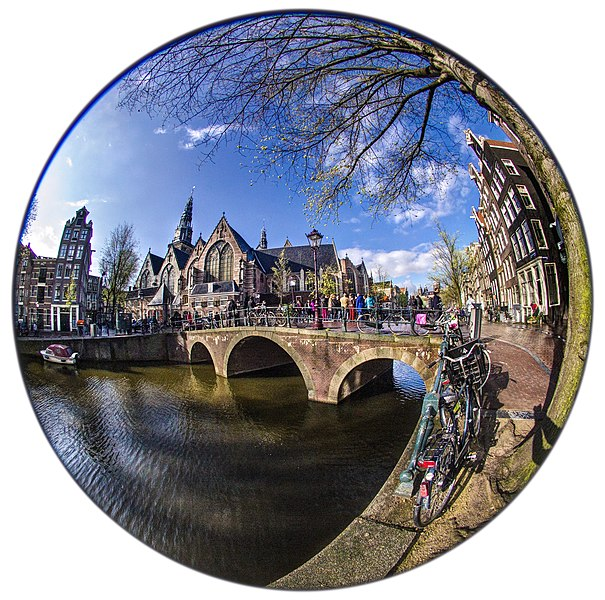
\includegraphics[width=1\columnwidth]{report1-img003.png} % Example image
	\caption{A photo taken with fisheye camera lens. The term fisheye was coined in 1906 by American physicist and inventor Robert W. Wood based on how a fish would see an ultrawide hemispherical view from beneath the water.}
\end{figure}

\clearpage

The camera also includes an IMU and an Intel® Movidius™ Myriad™ 2 Vision Processing Unit \href{https://www.intel.com/content/www/us/en/products/details/processors/movidius-vpu.html}{[14]}. All of the V‑SLAM algorithms run directly on the VPU, allowing for low latency and efficient power consumption. The T265 has been extensively tested and validated for performance, providing under 1\% closed loop drift under intended use conditions.\footnote{An ideal operating environment for the T265 has a reasonable number of fixed, distinct visual features in view as well as light levels higher than 15 lux \href{https://www.intelrealsense.com/tracking-camera-t265/}{[1]}. } It also offers sub 6ms latency between movement and reflection of movement in the pose. This is fast enough for even highly-sensitive applications such as Augmented and Virtual Reality. 

\section{Method}

\subsection{Setting up the environment}

Since Ubuntu 20.04 (focal fossa) and ROS noetic were utilized for the purposes of this project, the latest versions of both of these operating systems were installed on a local machine. This machine runs on 16GB of DDR-4 RAM and an average processor. It is equipped with a dedicated Nvidia graphics card utilizing 6GB of V-RAM memory. Most of the sotftware used for the purposes of this project exploits hardware acceleration in some way. Whenever this is the case, it will be specifically stated.

\subsection{Configuring the cameras}

The first necessary step to configure the cameras is the installation of the oficcial Intel® RealSense™ SDK 2.0 for ubuntu 20.04 . It was easily and successfully installed. Both of the cameras worked as intended while using the SDK.
\subsubsection{Configuring the T265 tracking camera}
It is worth noting that the T265 tracking module was experiencing fatal issues when connected to the PC via USB 3.0. The errors disappeared when it was connected via USB 2.0. A warning stating that connection over USB 2.0 could give unreliable results was being displayed nevertheless.

According to \href{https://support.intelrealsense.com/hc/en-us/community/posts/360038384494-USB-2-for-T265}{[15]} there are various user reports of pose drift when using the T265 with USB 2.0 connections, due to lower data transfer rate. 

This was tested experimentally. The camera was initially connected to a USB 2.0 port. It was then moved so as to follow a perfectly square path with a side of 70cm in length, on a level surface. The sides of the square as computed by the T265 tracking camera were measured using the realsense-viewer GUI. Then they were compared to the ground truth (70cm). The error 

\( error = \frac{| length\_measured - real\_length |} {real\_length} \)

was computed for each side. Then the mean of those errors was computed. The experiment was repeated four times. The experiment was then repeated four times with the camera connected over USB 3.0. For each experiment, the camera returned to its initial position as expected when following a square trajectory. However, a deviation between the initial and final position was observed in realsense-viewer. This closed loop drift was also measured. The results are documented in table 2. The experimental layout is shown in Figure 4.

\begin{figure}[h] % [h] forces the figure to be output where it is defined in the code (it suppresses floating)
	\centering
	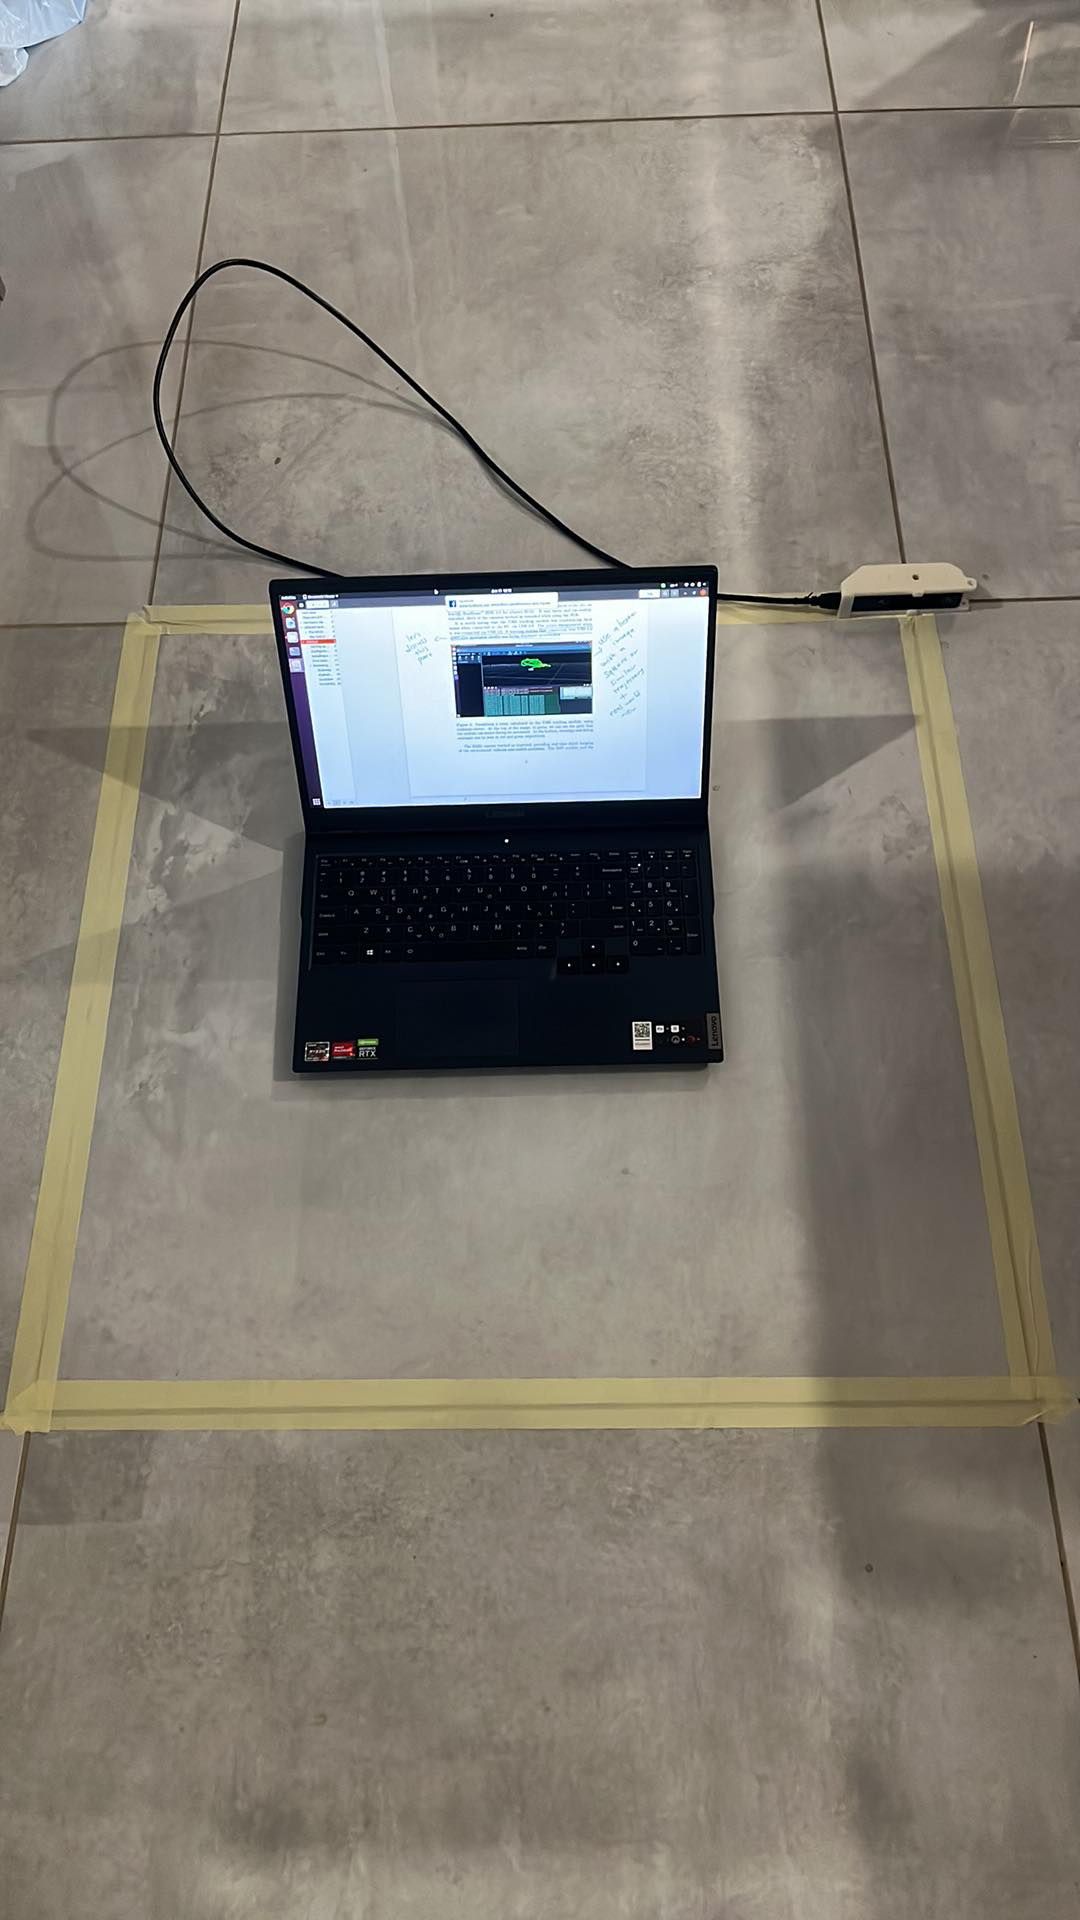
\includegraphics[width=1\columnwidth]{report1-img026.jpg} % Example image
	\caption{The experiments took place on a flat, smooth surface. The trajectory that the camera followed is marked by white tape.  }
\end{figure}

\begin{table}[h] % [h] forces the table to be output where it is defined in the code (it suppresses floating)
\noindent\makebox[\textwidth]{%
    \begin{tabular}{l l l l l}
        		\toprule
        		\textbf{Connection} & \textit{\vtop{\hbox{\strut 1st mean}\hbox{\strut error(cm)}}} & \textit{\vtop{\hbox{\strut 2nd mean}\hbox{\strut error(cm)}}} & \textit{\vtop{\hbox{\strut 3rd mean}\hbox{\strut error(cm)}})} & \textit{\vtop{\hbox{\strut 4th mean}\hbox{\strut error(cm)}}}\\
        		\midrule
        		USB 2.0 & 1.1 & 0.8 & 3.2 & 2.1\\
        		USB 3.0 & 0.7 & 0.5 & 0.8 & 3.2\\
        		\bottomrule
    \end{tabular}
}
\end{table}

\begin{table}[h] % [h] forces the table to be output where it is defined in the code (it suppresses floating)
\noindent\makebox[\textwidth]{%
    \begin{tabular}{l l l}
        		\toprule
        		\textbf{Connection} & \textit{Total mean (\%)} & \textit{\vtop{\hbox{\strut closed loop}\hbox{\strut drift(\%)}}} \\
        		\midrule
        		USB 2.0 & 2.57 & 0.8 \\
        		USB 3.0 & 1.8 & 0.4 \\
        		\bottomrule
    \end{tabular}
}

\caption{Tracking accuracy and closed loop drift of the T265 measured on a square trajectory.}
\end{table}

There is a measurable improvement in the accuracy of the tracking camera when connecting it with USB 3.0. In addition, it was a frequent occurrence that the camera would momentarily lose tracking when connected over USB 2.0, as shown in Figure 5. While connecting the camera via USB 3.0 solved this issue, it is evident that the trajectory is still far from perfect, as shown in Figure 6 and verified by the errors in Table 2.

\begin{figure}[h] % [h] forces the figure to be output where it is defined in the code (it suppresses floating)
	\centering
	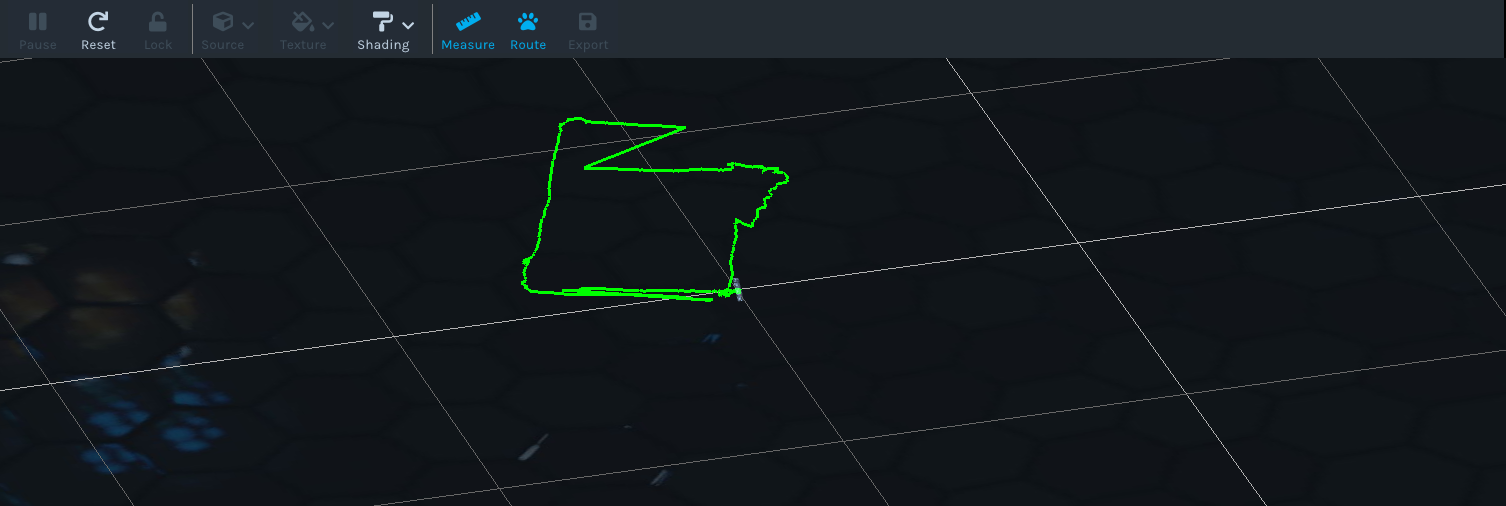
\includegraphics[width=1\columnwidth]{report1-img027.png} % Example image
	\caption{Visualizing a route calculated by the T265 tracking module connected via USB 2.0, using realsense-viewer. The camera followed a perfectly square path, with a side of 70cm in length. The camera lost track of its position at one point, which is visible as a spike on its marked trajectory. }
\end{figure}

\begin{figure}[h] % [h] forces the figure to be output where it is defined in the code (it suppresses floating)
	\centering
	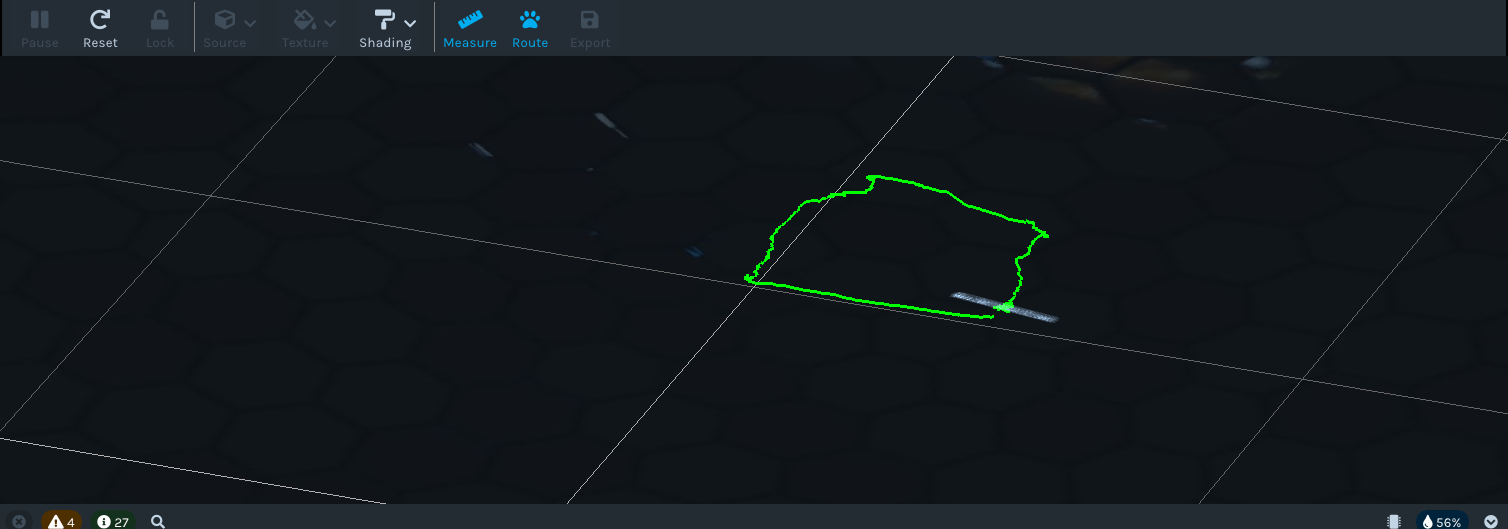
\includegraphics[width=1\columnwidth]{report1-img028.png} % Example image
	\caption{Visualizing a route calculated by the T265 tracking module connected via USB 3.0, using realsense-viewer. The camera did not lose track of its position. The shape of the calculated path does not match the real path perfectly. }
\end{figure}

\clearpage


\subsubsection{Configuring the D435i depth camera}

The D435i camera worked as expected, providing real time depth imaging of the environment. The IMU returned accurate data regarding the translation and rotation of the cameras in real time, with low latency.

The camera was stationed 1 meter away from the base of a wooden staircase. Distances were accurately visualised in the depth stream. The individual stairs can be clearly distinguished in the depth image, as can be seen in Figure 8.

The accelerometer and gyro streams from the D435i's IMU module can be seen in Figure 9. Both of the sensors were responsive to camera movement. 



Intel claims that the D435i camera has a depth error of less than 2\% at distances not greater than 10 meters \href{https://www.intelrealsense.com/depth-camera-d435i/}{[2]}. To test this, the camera was stationed one meter away from the first stair of the wooden staircase seen in figure 8 and 1 meter above the floor. For the first seven stairs, we measured the distance from the camera to the lower right corner of each stair and compared it to the distance that the camera measured, which was acquired using the realsense-viewer measure tool. The error in \% is plotted in Figure 10. The error does not exceed the 2\% threshold even though the distance of the last stair measured is more than 3 meters.

\clearpage

\begin{figure}
\begin{subfigure}{0.5\textwidth}
  \centering
  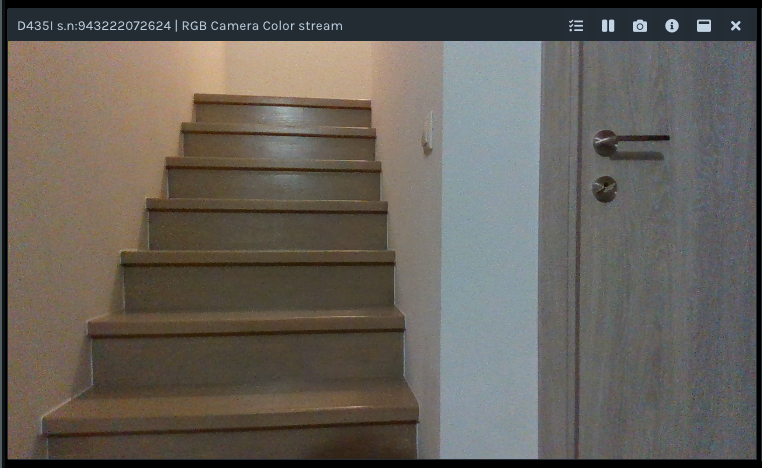
\includegraphics[width=0.95\linewidth]{report1-img029.png}
  \caption{}
  \label{fig:sfig1}
\end{subfigure}%
\begin{subfigure}{0.5\textwidth}
  \centering
  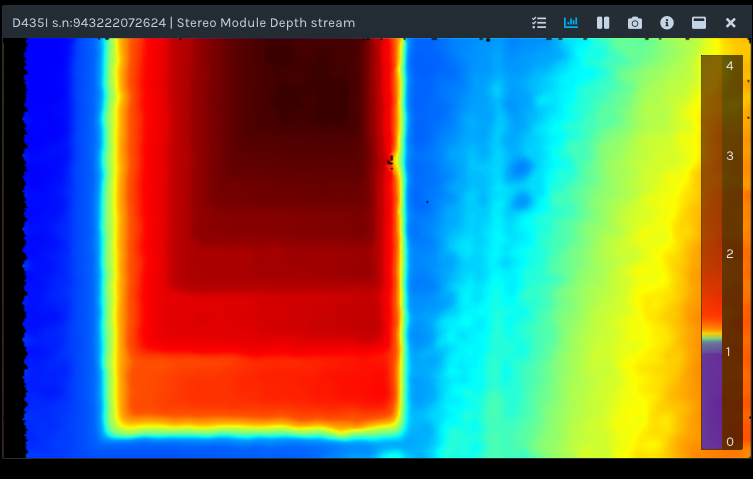
\includegraphics[width=0.95\linewidth]{report1-img030.png}
  \caption{}
  \label{fig:sfig2}
\end{subfigure}
\caption{The realsense-viewer environment with the D435i camera. Observable at 8a is the full-HD color stream of the staircase. At 8b, the depth stream along with a color depth scale can be seen. The base of the staircase is green in color which means that it is correctly registered as being 1 meter away from the camera.}
\label{fig:fig}
\end{figure}

\begin{figure}[h] % [h] forces the figure to be output where it is defined in the code (it suppresses floating)
    \centering
	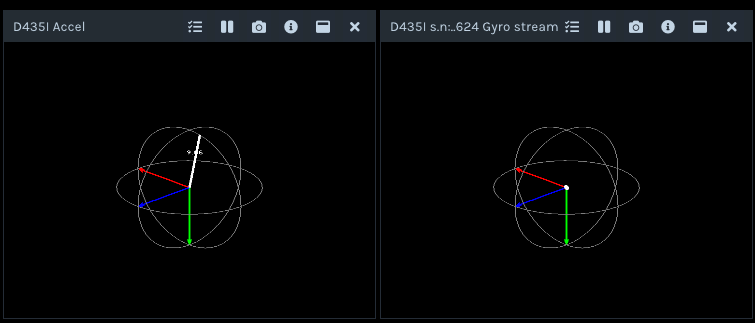
\includegraphics[width=\textwidth,height=\textheight,keepaspectratio]{report1-img031.png} % Example image
	\caption{The D435i camera comes with an IMU module and thus produces accelerometer and gyro streams. }
\end{figure}

\begin{figure}[h] % [h] forces the figure to be output where it is defined in the code (it suppresses floating)
    \centering
    \textbf{D435i Depth Error}\par\medskip
	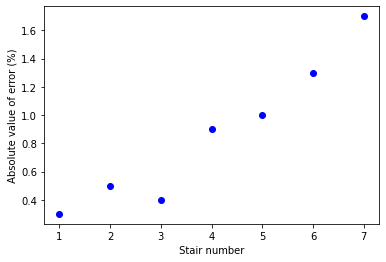
\includegraphics[width=\textwidth,height=\textheight,keepaspectratio]{report1-img032.png} % Example image
	\caption{Depth error in \% for the first seven stair steps. The error remains less than 2\% for distances less than 4 meters.}
\end{figure}

\clearpage

\subsection{Installing a Ros Wrapper}

A C++ ROS Wrapper is a design pattern that uses one C++ class to expose a ROS interface for an underlying, or wrapped, piece of code. Each ROS Wrapper is instantiated inside of a ROS Node, reads its configuration from the Parameter Server, and often publishes/subscribes to information on Topics using a namespace passed to them on construction. Any number of ROS Wrappers may be instantiated within a single ROS Node and can be linked together via both their ROS interfaces and their C++ APIs.\href{http://wiki.ros.org/navigation/ROS_Wrappers}{[16]}

Regarding the ROS Wrapper for the realsense cameras, it is a way for the realsense cameras to publish data over ROS topics so that they can be used by other ROS nodes or services.
Two installation methods for the realsense ROS Wrapper are available:

The first one is installing the ROS Distribution of the wrapper and the second one is installing the Intel® RealSense™ Distribution. The first one is the simplest method. However, as stated in the installation website, the libraries installed with the ROS Distribution might be deprecated and the communication protocol used for transmitting data over ROS is less stable. \href{https://github.com/IntelRealSense/realsense-ros}{[12]}

Thus, for this project, the  Intel® RealSense™ Distribution was installed. Note that the .travis.yml file which is in the package, should be consulted during this type of installation. First the following packages should be updated:

\begin{lstlisting}[language=bash]
  $ sudo apt install "$_python"-rosdep -y
  $ sudo rosdep init
  $ rosdep update
  $ sudo apt-get install ros-$_ros_dist-cv-bridge -y
  $ sudo apt-get install ros-$_ros_dist-image-transport
  $ sudo apt-get install ros-$_ros_dist-tf -y
  $ sudo apt-get install ros-$_ros_dist-diagnostic-updater -y
  $ sudo apt-get install ros-$_ros_dist-ddynamic-reconfigure -y

\end{lstlisting}

\begin{verbatim}
Where in our case "$_python" = python3 and $_ros_dist = noetic
\end{verbatim}

Then, a catkin workspace needs to be created:

\begin{lstlisting}[language=bash]
  $ mkdir -p ~/catkin_ws/src
  $ cd ~/catkin_ws/src/
\end{lstlisting}

The latest Intel® RealSense™ ROS Wrapper needs to be cloned into the workspace:

\begin{lstlisting}[language=bash]
  $ git clone https://github.com/IntelRealSense/realsense-ros.git
  $ cd realsense-ros/
  $ git checkout `git tag | sort -V | grep -P "^2.\d+\.\d+" | tail -1`
  $ cd ..
\end{lstlisting}

Then, the packages need to be compiled and installed:

\begin{lstlisting}[language=bash]
  $ catkin_init_workspace
  $ cd ..
  $ source ~/catkin_ws/devel/setup.bash
  $ catkin_make clean
  $ catkin_make -DCATKIN_ENABLE_TESTING=False -DCMAKE_BUILD_TYPE=Release
  $ catkin_make install
\end{lstlisting}

Finally, the setup.bash in the workspace needs to be sourced:

\begin{lstlisting}[language=bash]
  $ source ~/catkin_ws/devel/setup.bash
\end{lstlisting}

The node that launches a single realsense camera is rs\_camera.launch and is located inside the realsense2\_camera package. It can be launched with: 

\begin{lstlisting}[language=bash]
  $ roslaunch realsense2_camera rs_camera.launch
\end{lstlisting}


\subsection{First tests over ROS}

The ROS Wrapper is essentially a ROS package named realsense-ros. With it, the realsense cameras can be used with ROS. It includes launch files which can be used to operate one or more of the cameras at the same time. The cameras were launched and tested first separately and then simultaneously.

By using the cameras with ROS, it should be noted that the T265 tracking camera has reduced functionality when used over USB 2.0. Odometry topics cannot be published. The error that appears mentions T265 connectivity:

\textit{[Error]: Streaming over USB 2.1 is unreliable, please use USB 3 or only stream poses.}

Odometry topics are necessary for implementing SLAM. Thus, connectivity issues should be resolved before proceeding. Such issues are considered common with this particular camera \href{https://support.intelrealsense.com/hc/en-us/community/posts/360033359193-T265-Device-not-detected}{[17]}.

After several tests with the T265 tracking camera, it was realised that the camera showed unexpected glitches when connected via USB 3.0. A USB 3.0 splitter hub was ordered in order to connect both of the cameras to a correct and identical type of port. The issue persisted nevertheless. 

Eventually, it turned out that the factory cable was faulty. A  new camera cable (USB micro-B) was used and the camera worked correctly over both USB 2.0 and USB 3.0 connections.

Inside the rs\_camera.launch file which can be used for launching the D435i camera, it was observed that most of the available topics are not published by default. The arguments enable\_depth, enable\_infra1, enable\_infra2, enable\_gyro and enable\_accel should be set to true, in order to enable the most important functionalities of the D435i camera. Namely, enabling the camera's infrared light emitters allows the cameras to use structured light to better register depth. The gyroscope and accelerometer topics can be used to improve odometry.

\begin{figure}[h] % [h] forces the figure to be output where it is defined in the code (it suppresses floating)
    \centering
	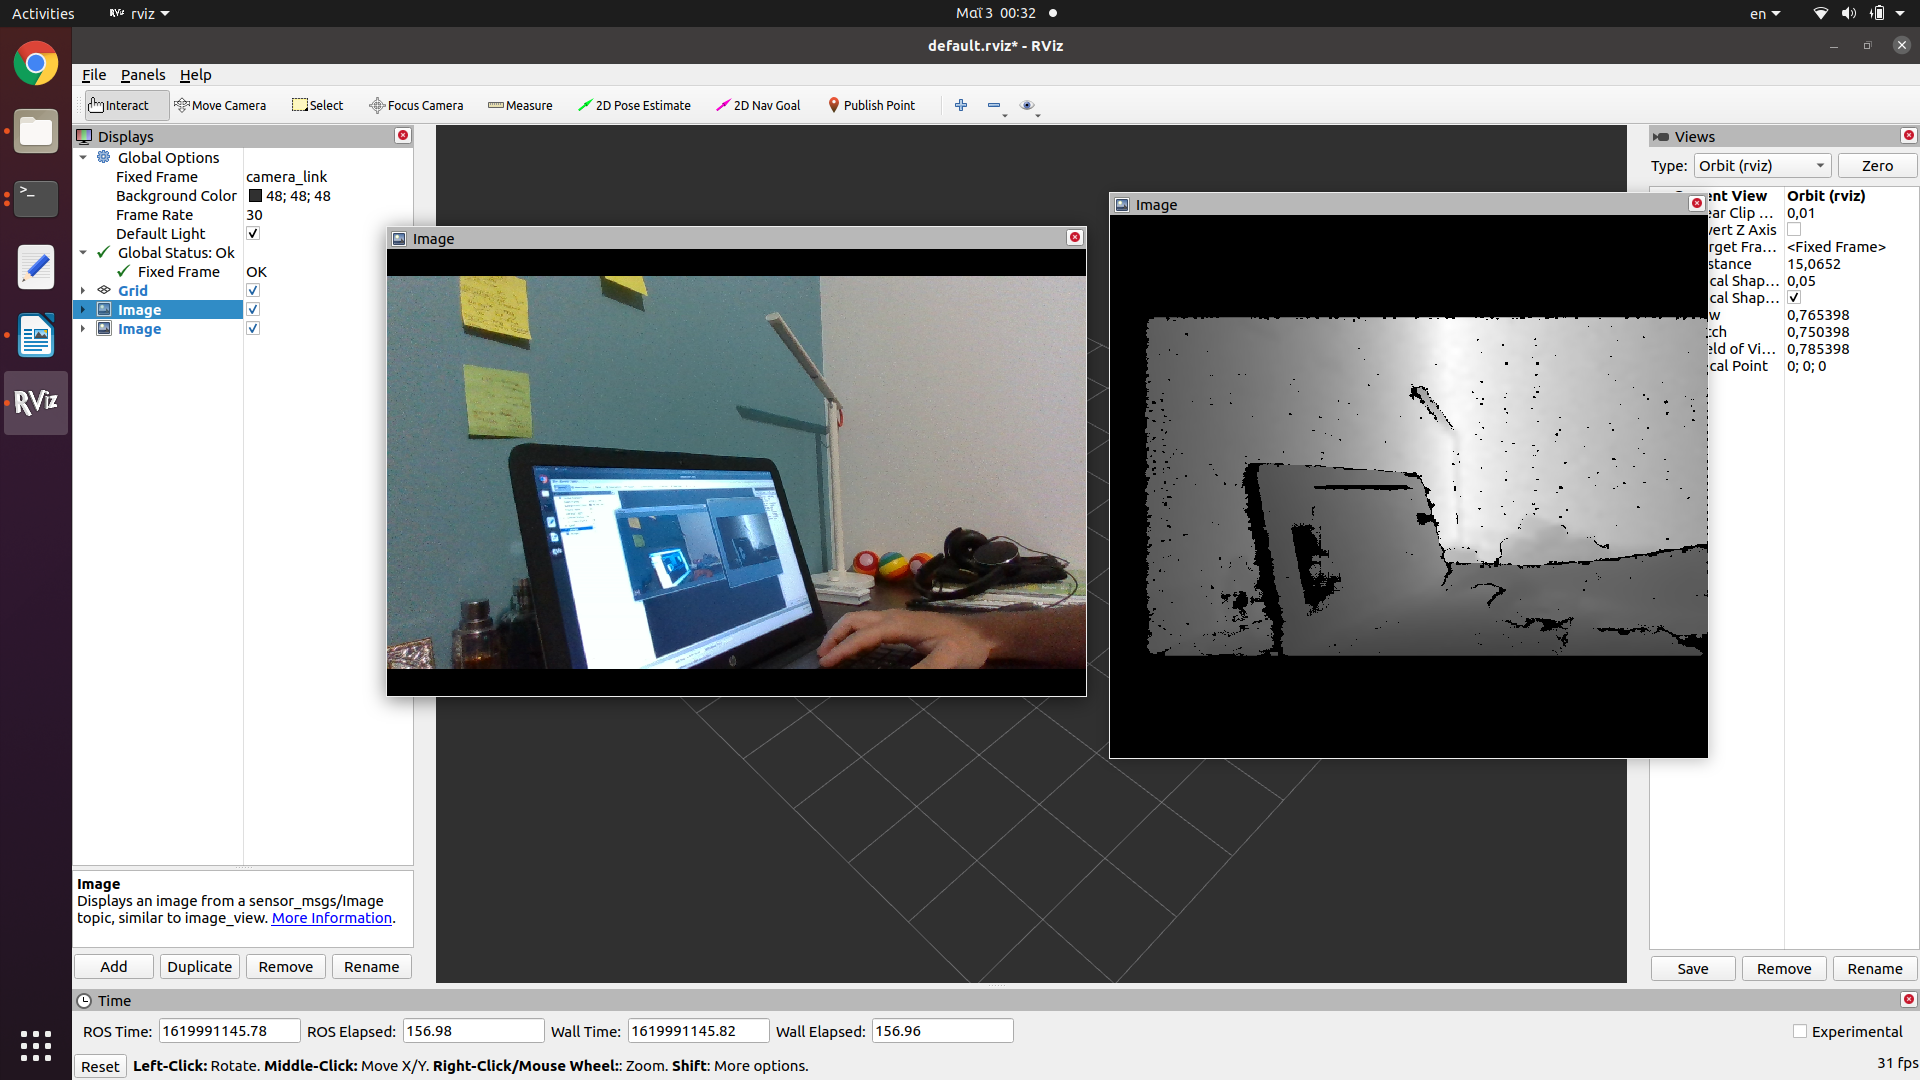
\includegraphics[width=\textwidth,height=\textheight,keepaspectratio]{report1-img008.png} % Example image
	\caption{Viewing the /color/image\_raw and /depth/image\_raw D435i topics in Rviz.}
\end{figure}

\begin{figure}[h] % [h] forces the figure to be output where it is defined in the code (it suppresses floating)
    \centering
	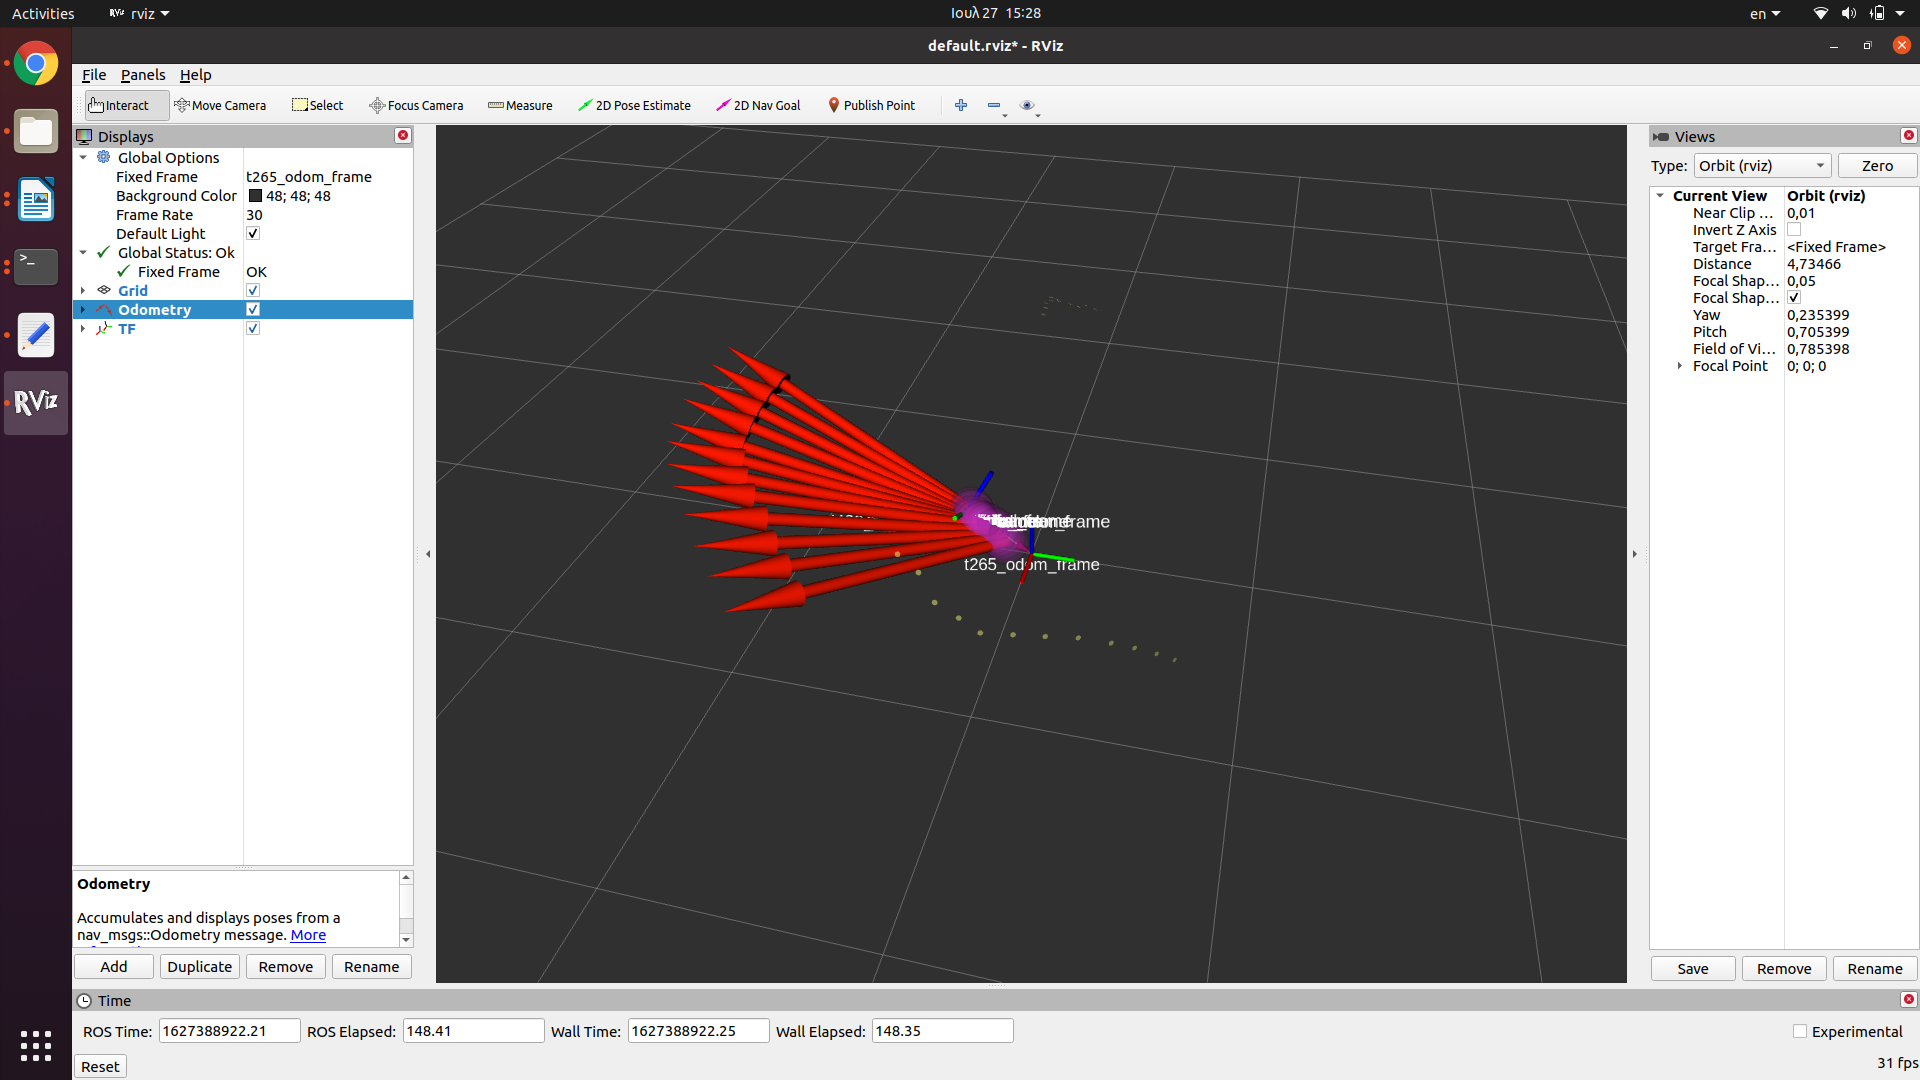
\includegraphics[width=\textwidth,height=\textheight,keepaspectratio]{report1-img009.png} % Example image
	\caption{The t265/odom/sample odometry topic. The points of the red arrows show the direction the camera faces. The arrow tail matches the camera's position over time. The purple spheres describe the positional uncertainty of the pose estimate. The little yellow dots describe the angular uncertainty of the pose estimate.}
\end{figure}

\clearpage

\subsection{Reviewing available software packages for the Elevation Mapping}

Three different packages were tested. Each package was used to create the elevation map of a wooden staircase. The experiment took place indoors, under artificial and steady lighting conditions. The cameras were stationed 1 meter far from the base of the staircase and were handheld and moving during the tests. 

\begin{figure}[h] % [h] forces the figure to be output where it is defined in the code (it suppresses floating)
    \centering
	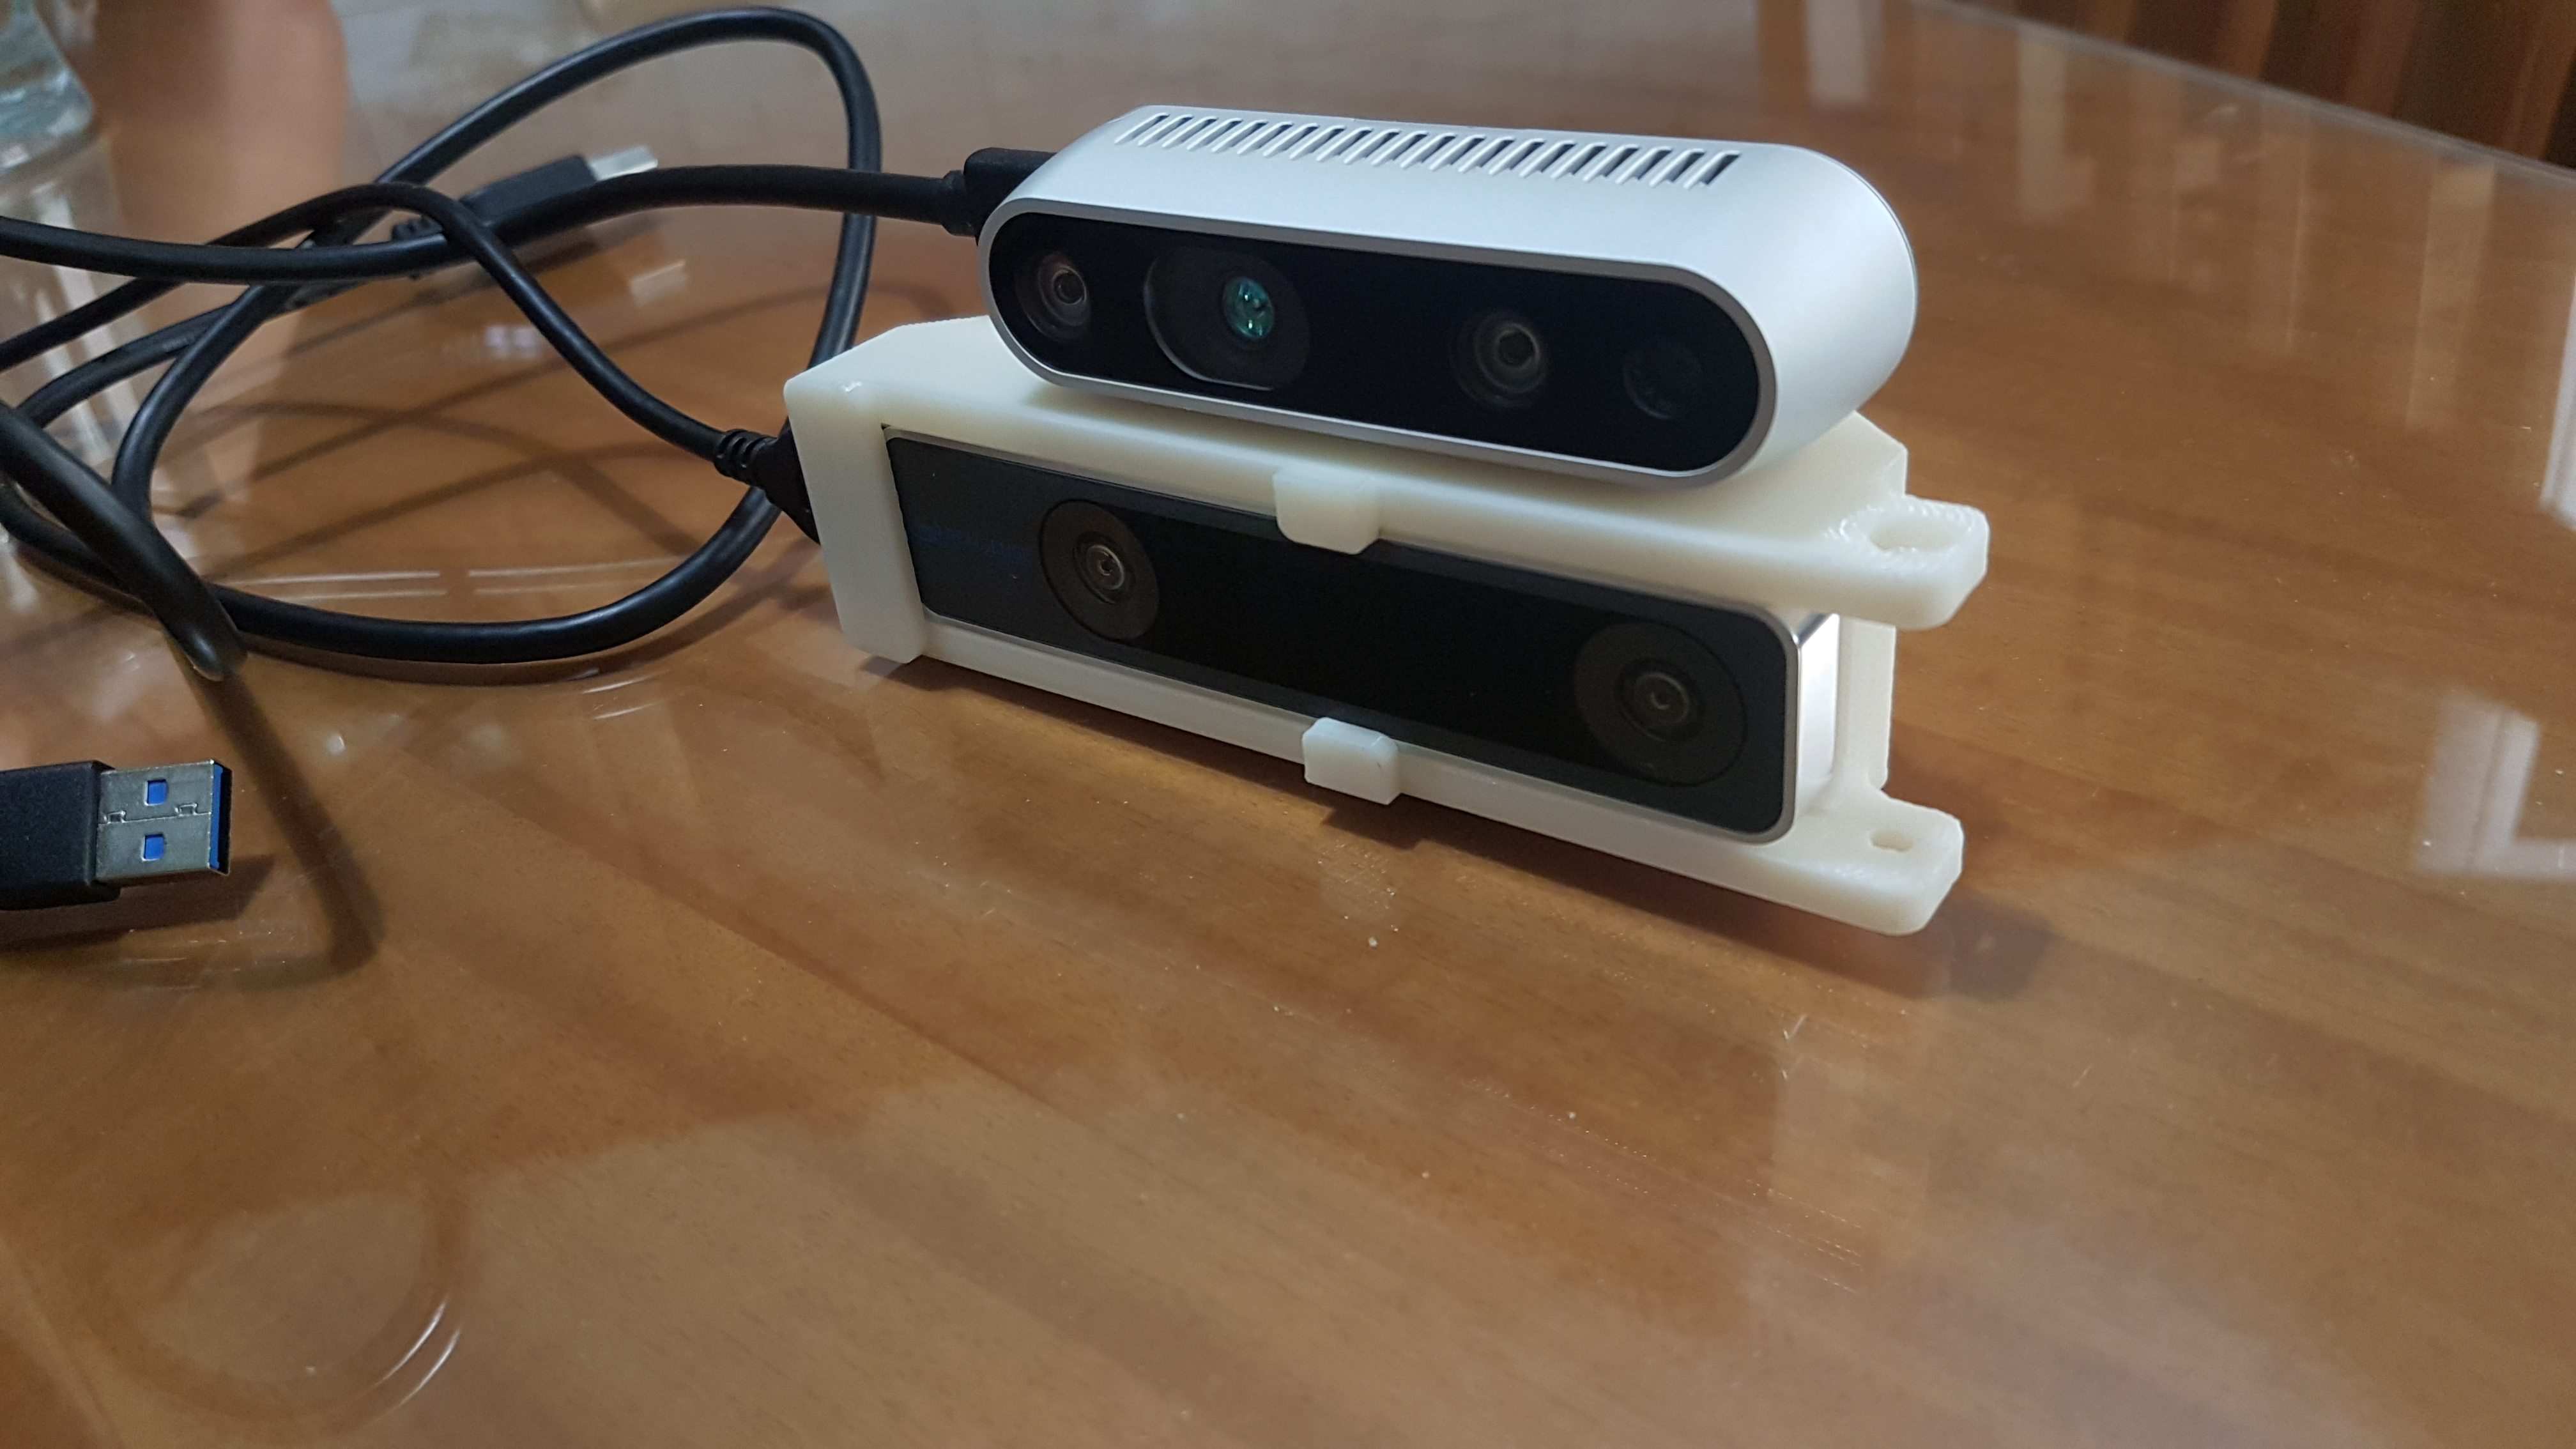
\includegraphics[width=\textwidth,height=\textheight,keepaspectratio]{report1-img010.jpg} % Example image
	\caption{The cameras were fastened on a special 3d printed mount. The static transform between the cameras corresponds to their positions on the mount.}
\end{figure}

\subsubsection{Rtabmap}

RTAB-Map (Real-Time Appearance-Based Mapping) is an RGB-D, Stereo and Lidar Graph-Based SLAM approach based on an incremental appearance-based loop closure detector. The loop closure detector uses a bag-of-words approach to determinate how likely a new image comes from a previous location or a new location. That means that each new acquired image is dissected into visual words. Similarly to how a text is dissected into words. 

For example, in the classic classification problem of labeling an email as spam or not spam, each email is parsed into words and one can deduce if the mail was spam or not spam solely by reviewing the frequency at which each word appeared. For instance, if the word “money” appeared more frequently in a target email than in the average email, then there was a large chance that the target email is spam.

Comparably, RTAB-Map parses each new frame into small homogenous pieces known as visual words. Then, it compares the frequency that each word appears in the newly acquired frame appears to a database consisting of data from previously acquired frames. If the newly acquired frame consists of similar visual words to a previously seen frame, then this bag-of-words approach determines that the new image comes from a location that has been visited before. This is known as accepting a loop closure hypothesis.

When a loop closure hypothesis is accepted, a new constraint is added to the map’s graph, then a graph optimizer minimizes the errors in the map. Namely, the information that the robot is currently in a place where it has been before is used to correct its calculated trajectory. 

A memory management approach is used to limit the number of locations used for loop closure detection and graph optimization, so that real-time constraints on large-scale environments are always respected. RTAB-Map can be used alone with a handheld stereo camera for 6DoF mapping. \href{http://introlab.github.io/rtabmap/}{[18]}

Rtabmap is a stable and well known package and can be used with structured light and stereo-depth cameras as well as with lidars and laser rangefinders. Recently, a version of the package for iOS devices has been released and produces high quality results paving the way for wider commercial use of the rtabmap algorithm. \href{https://www.youtube.com/watch?v=rVpIcrgD5c0}{[19]}

\newpage
\textit{Measuring and testing}
\bigskip

The realsense cameras along with rtabmap seem to do a very good job at producing an accurate pointcloud even when being moved vigorously while forming the map. Rviz offers a useful measurement tool. This enables the user to compare distances as perceived by the cameras with their real life counterparts. Handholding the camera at about one meter away from the base of a wooden staircase, the staircase was viewed from different angles, until an almost complete map of the staircase was generated. 

\begin{figure}[h] % [h] forces the figure to be output where it is defined in the code (it suppresses floating)
    \centering
	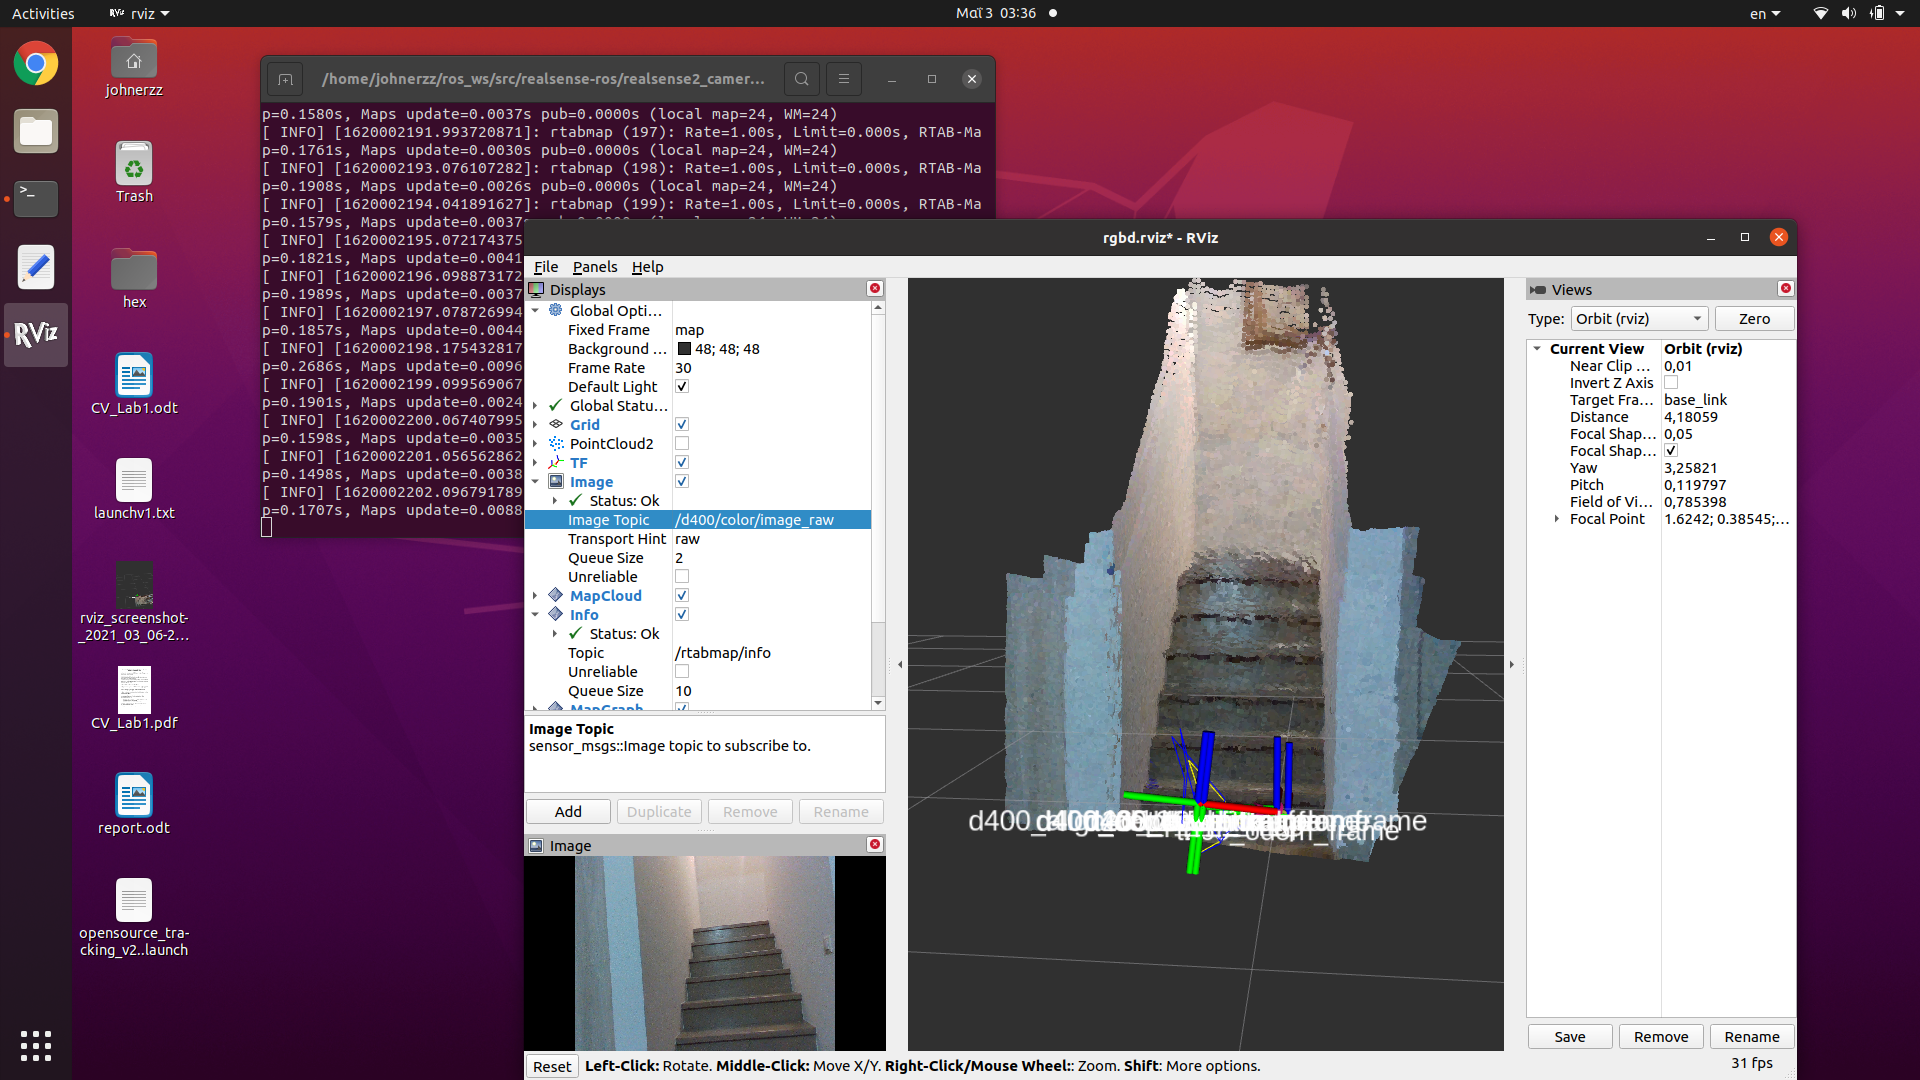
\includegraphics[width=\textwidth,height=\textheight,keepaspectratio,trim={18cm 0 4cm 8cm},clip]{report1-img011.png} %
\end{figure}

\begin{figure}[h] % [h] forces the figure to be output where it is defined in the code (it suppresses floating)
    \centering
	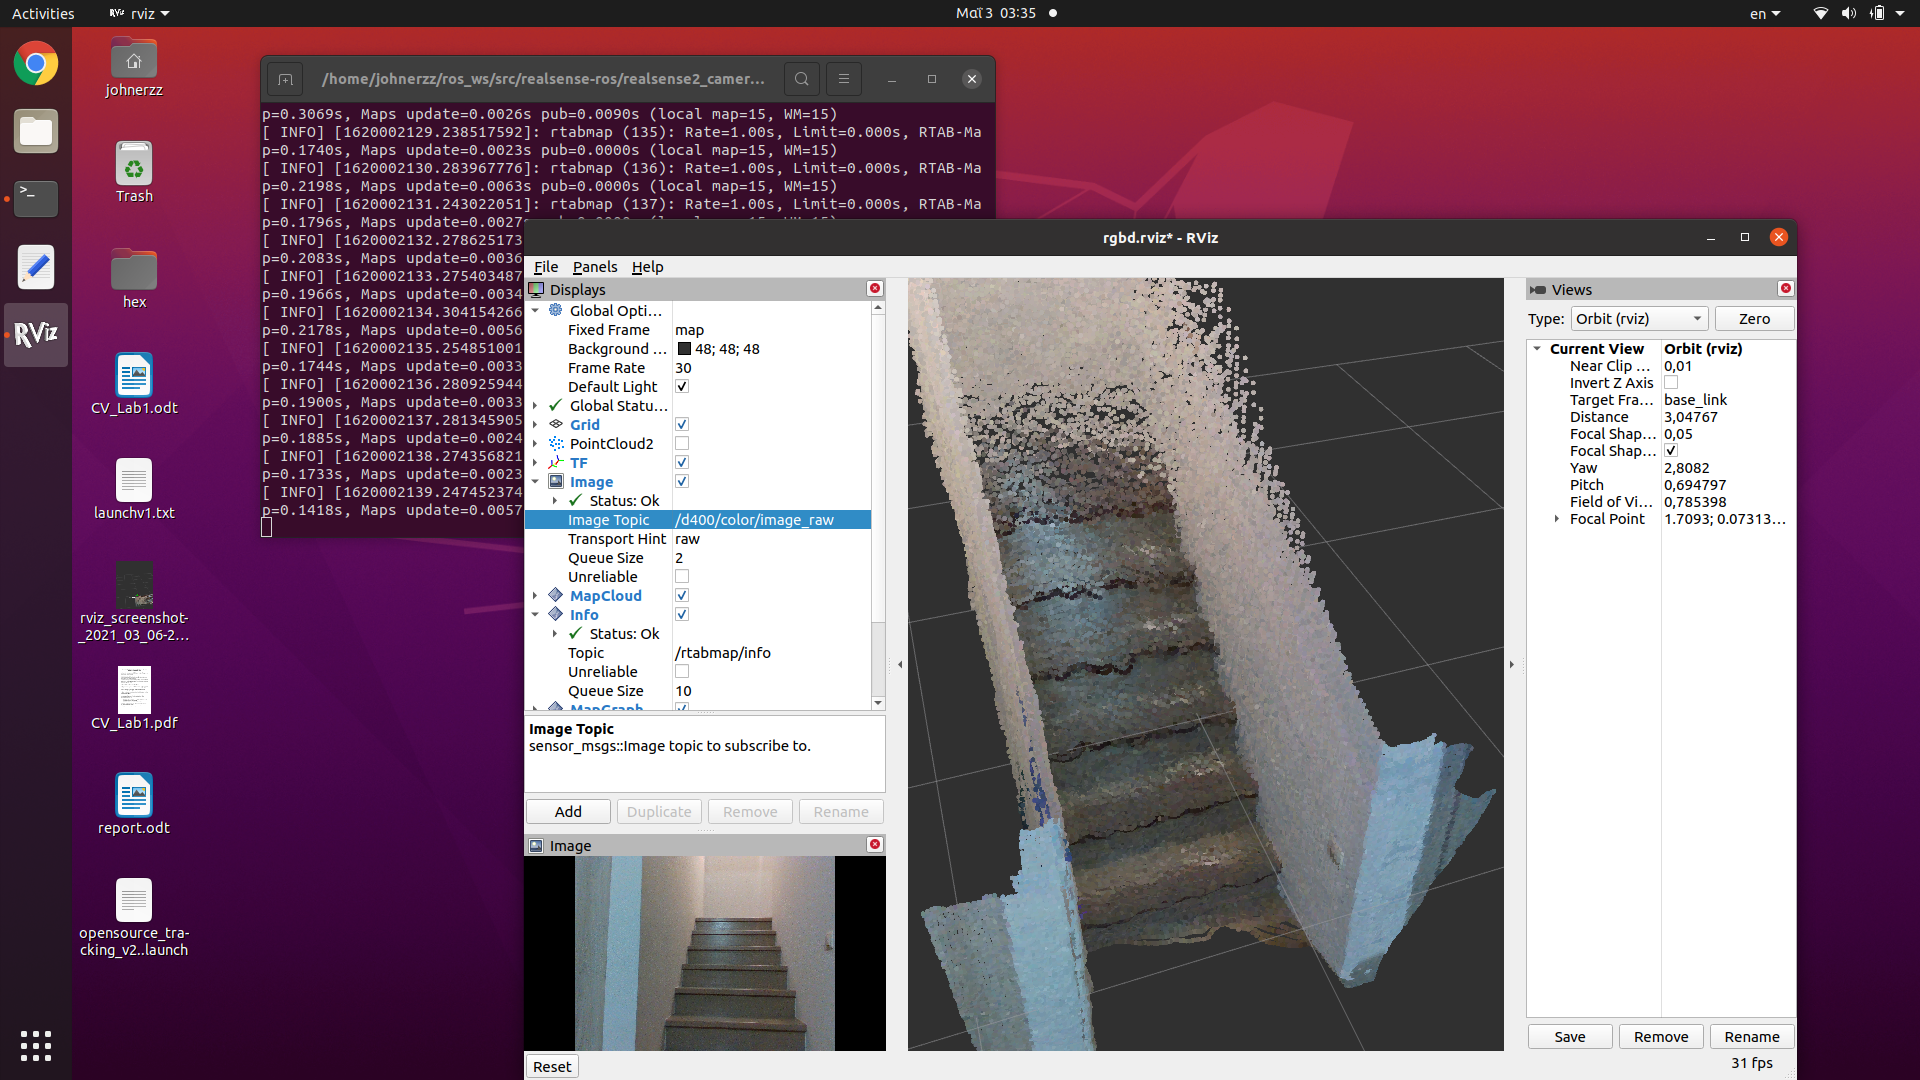
\includegraphics[width=\textwidth,height=\textheight,keepaspectratio,trim={18cm 0 4cm 8cm},clip]{report1-img013.png} %
	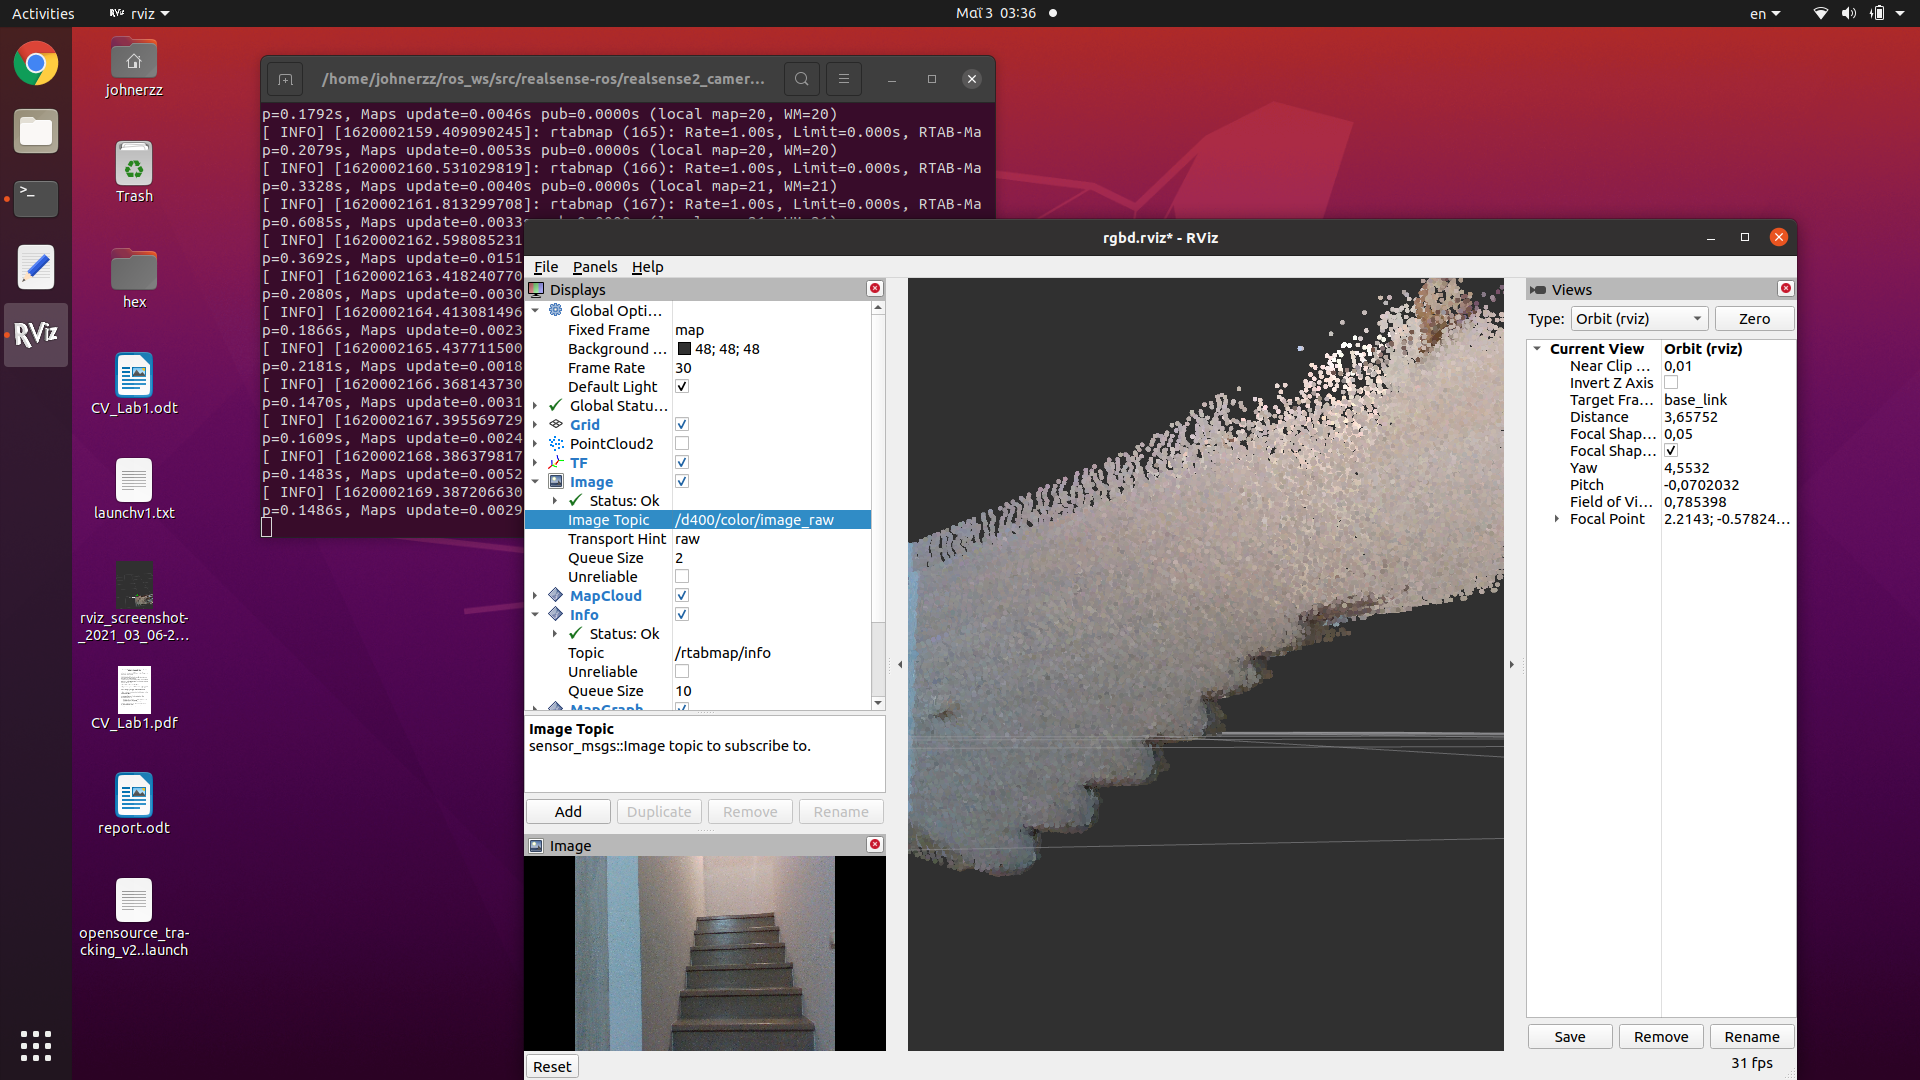
\includegraphics[width=\textwidth,height=\textheight,keepaspectratio,trim={18cm 0 4cm 8cm},clip]{report1-img012.png} %
	\caption{Elevation Mapping of a staircase made with Rtabmap. Pointcloud viewed from various angles in rviz. }
\end{figure}

\clearpage
\bigskip
\bigskip
\bigskip
\bigskip


The height of each stair step was measured as registered in the map made with rtabmap and was then compared to the real height of the stair steps which is 20cm. Subtracting the measured value from the real value gives us the measurement error. We then plot the absolute value of this error for the first seven stair steps.

With an average error of about 4.6\% and given that the measurements for the real dimensions of the objects were made by hand, it can be deduced that this setup is capable of producing usable volumetric measurements. The measurements are less accurate for distant targets. This is reflected in this experiment as the fifth and sixth stair steps are measured rather inaccurately and appear noisy on the elevation map. 

\begin{figure}[h] % [h] forces the figure to be output where it is defined in the code (it suppresses floating)
    \centering
    \textbf{Rtabmap Volumetric Error}\par\medskip
	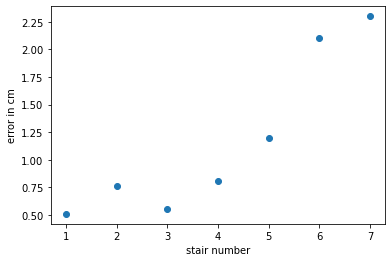
\includegraphics[width=\textwidth,height=\textheight,keepaspectratio]{report1-img014.png} %
	\caption{Absolute error value of stair height in centimeters for the first seven stair steps. }
\end{figure}

\clearpage

Nevertheless, the pointcloud that Rtabmap produces with the current setup is dense and the localization of the cameras was not lost during any of our experiments. Using a detection rate of 10Hz - which means that the algorithm would check if the cameras are viewing a scene that has been viewed in the past (loop closure) ten times every second – it was observed that the node ran smoothly in real time albeit being a resource-intensive procedure. Note that there is a significant performance difference in RTAB-Map between the entire support chain (Eigen, OpenCV, VTK, and especially the feature detectors) being built with CUDA support versus without. Making use of a library that uses CUDA, is essentially using CUDA and  RTAB-Map is a package that is built with GPU acceleration in mind.

\subsubsection{Anybotics Elevation Mapping}

Anybotics Elevation Mapping is a ROS package developed for elevation mapping with a mobile robot. The software is designed for (local) navigation tasks with robots which are equipped with a pose estimation (e.g. IMU and odometry) and a distance sensor (e.g. structured light (Kinect, RealSense), laser range sensor, stereo camera) \href{https://github.com/ANYbotics/elevation_mapping}{[20]}. 

Achieving localization using proprioceptive sensing means that the estimates of the
position and yaw-rotation of a mobile robot accumulate uncertainty and drift over time in comparison to their real values. For example, when using using wheel odometry, a slight slip of one or both of the wheels will cause the calculated position and orientation of the robot to diverge from the real ones. If such divergences are not corrected, they accumulate over time and accurate localization is not achievable. Namely, the position and yaw-rotation remain unobservable.

A common approach to solve this problem is loop closure. Loop closure is the recognition of when the robot has returned to a previously mapped region (through, for example, recognizing previously seen visual features in the environment) and the use of this information to reduce the uncertainty in the
map estimate. Loop closure can be implemented using pose graph optimization, which is what Rtabmap does.

Instead of tackling the accumulation of uncertainty by implementing loop-closure, the algorithm from Anybotics produces an elevation map that is limited around the robot (robot-centric mapping). At any time, the robot-centric elevation map is a local representation of the surrounding terrain, meaning that the observed regions in front of the robot have the highest accuracy, while ‘older’, previously seen parts of the map accumulate uncertainty and ‘melt’ into each other.

The resulting probabilistic terrain is a is a grid-based elevation map consisting of individual cells. When the map is needed for further processing, a map fusion process creates a consistent estimate of the terrain map together with an uncertainty interval.
\href{https://www.research-collection.ethz.ch/bitstream/handle/20.500.11850/272110/fankhauser2018.pdf?sequence=1&isAllowed=y}{[21]}. 

This software comes with multiple dependencies. The following software needs to be installed before installing the package itself:

\begin{itemize}
    \item Grid Map (grid map library for mobile robots)
    \item kindr (kinematics and dynamics library for robotics)
    \item kindr\_ros (ROS wrapper for kindr)
    \item Point Cloud Library (PCL) (point cloud processing)
    \item Eigen (linear algebra library)
\end{itemize}

After installing all the dependencies, the package itself was installed by cloning the latest version from the official github repository in our ROS workspace and building it according to the instructions. 

There are two tools for building ROS workspaces: catkin\_make and catkin build. The authors of the elevation mapping package suggest building with catkin build. To do that, the catkin python tools need to be installed:

\begin{lstlisting}[language=bash]
    $ sudo apt install python3-catkin-tools python3-osrf-pycommon
\end{lstlisting}

After building with catkin build, then:

\begin{lstlisting}[language=bash]
    $ roscd elevation_mapping
    $ catkin build --catkin-make-args run_tests -- --this
    $ rostest elevation_mapping elevation_mapping.test -t
\end{lstlisting}

Those tests function as a diagnostic tool to ensure that everything was installed correctly.

\bigskip

\textit{Testing in simulation}

\bigskip

Before attempting to configure the package to work with our cameras, the package was tested in a simulated environment. This makes it possible to study how the algorithm would perform with a perfect depth sensor in a noiseless environment. The turtlebot simulated robot was used in a simulated house environment.


\begin{figure}[h] % [h] forces the figure to be output where it is defined in the code (it suppresses floating)
    \centering
	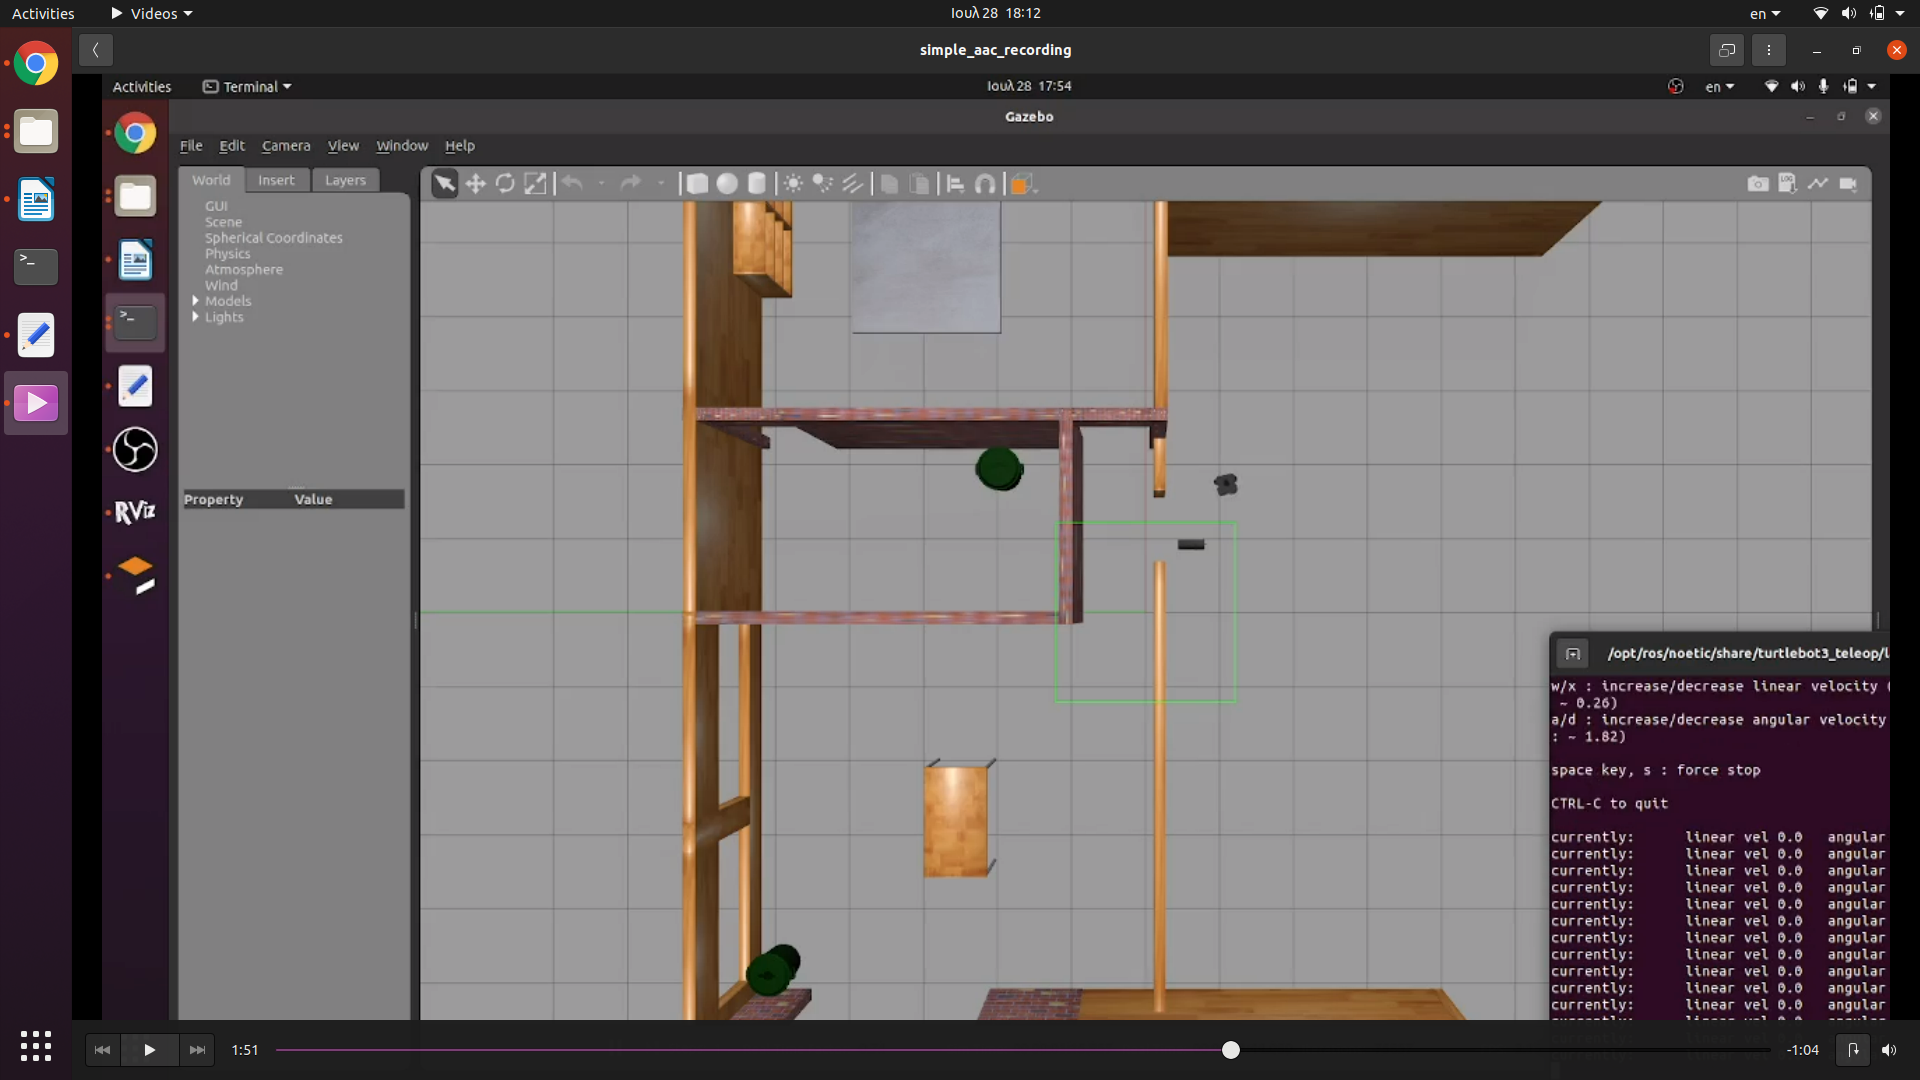
\includegraphics[width=\textwidth,height=\textheight,keepaspectratio]{report1-img015.png} %
	\caption{The simulated house environment as seen in Gazebo ROS. }
\end{figure}

The resulting map was a near perfect elevation map as was expected with a simulated setup. The map was being generated in real time in a smooth and consistent manner, but at a lower frequency than the one observed with rtabmap. Namely, the mean mapping frequency was measured to be lower than 2 Hz. 

\begin{figure}[h] % [h] forces the figure to be output where it is defined in the code (it suppresses floating)
    \centering
	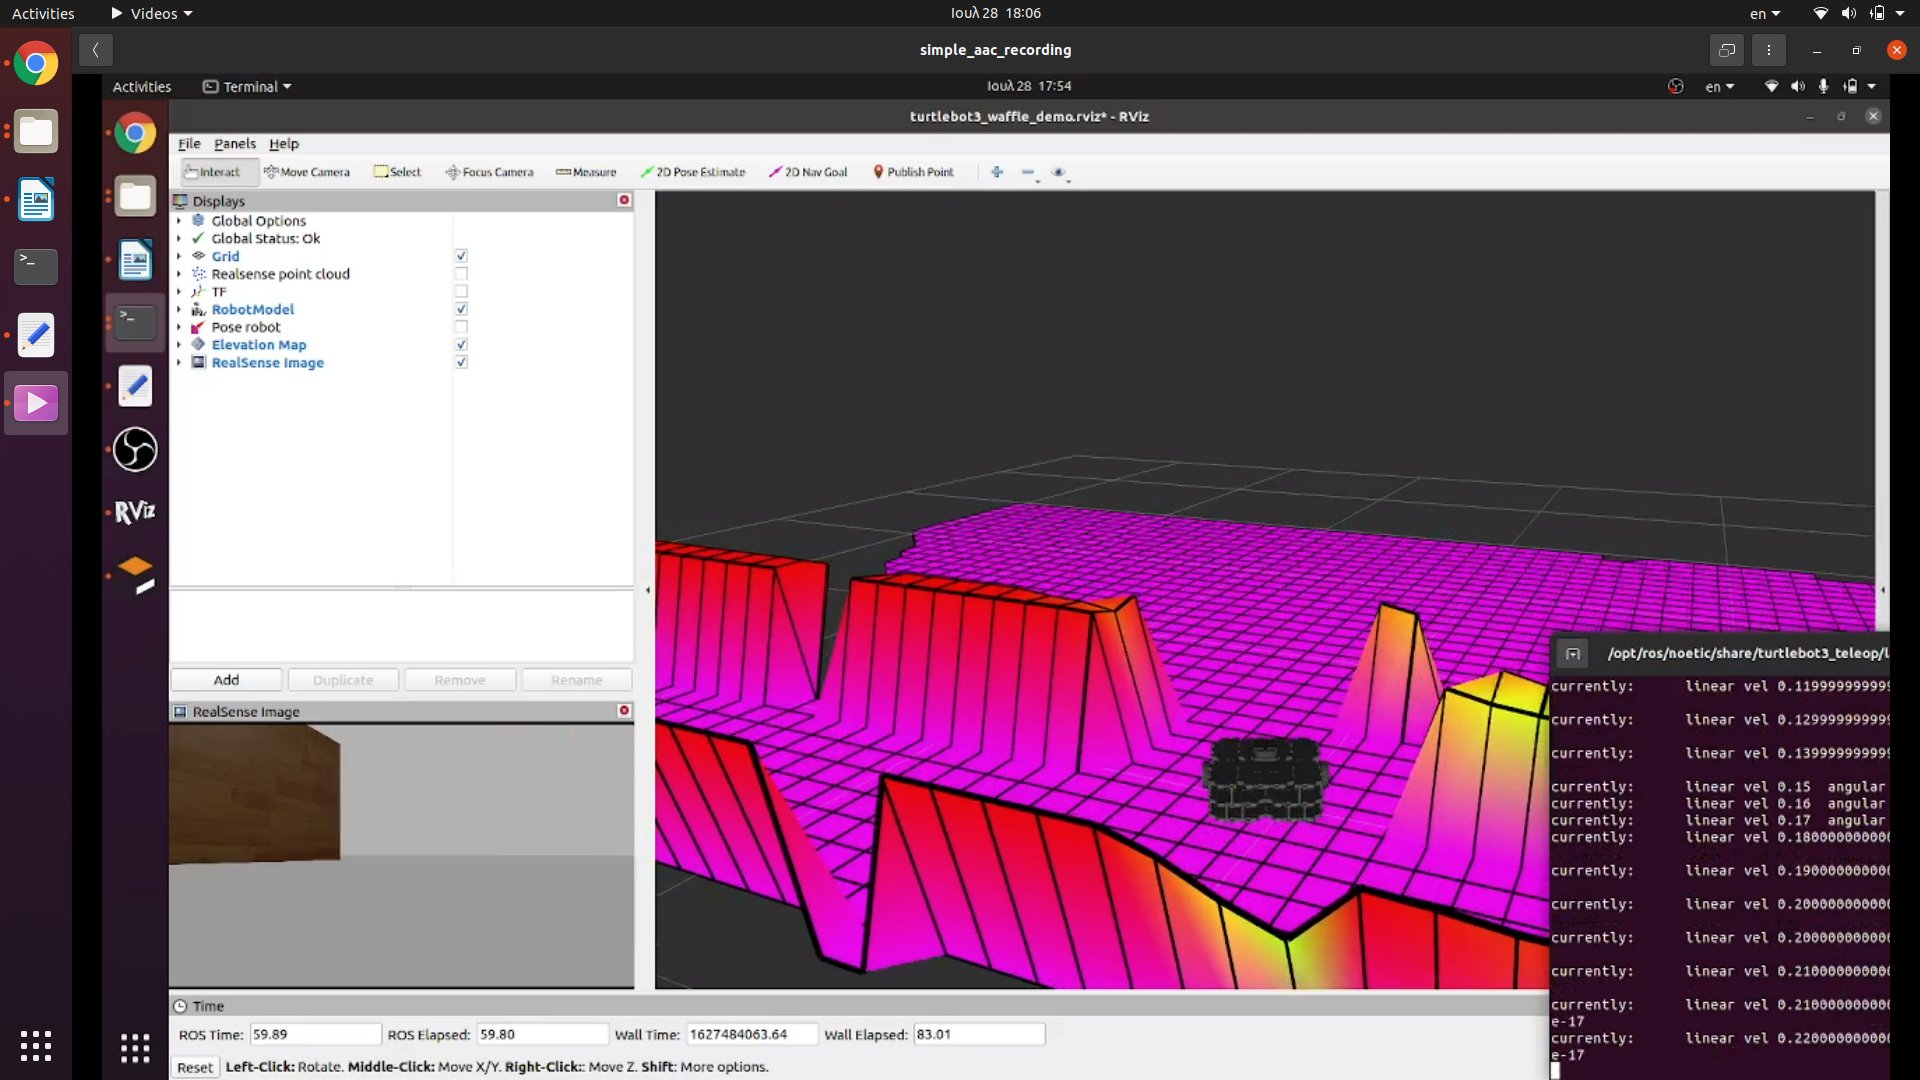
\includegraphics[width=\textwidth,height=\textheight,keepaspectratio]{report1-img016.png} %
	\caption{The elevation map of the simulated house as seen in Rviz. }
\end{figure}

\bigskip
\clearpage

\textit{Testing with the real cameras}

\bigskip

Next, the package was configured to work with the D435i and T265 cameras. A launch file was created to launch both cameras with the parameters required for the software to run. The software also required a pose instead of a TF transform so the tf\_to\_pose\_publisher.py script was used to publish the pose taken from the t265\_odom\_frame tf transform that the T265 produces. Finally Rviz is launched with the recommended arguments that were also used in the turtlebot simulated demo.

A .yaml configuration file was then written to provide the elevation mapping node with the topics and parameters it would read to generate the map. The "/d435/depth/color/points" pointcloud topic from the D435i camera and the "t265\_odom\_frame" transform topic from the T265 camera were ultimately chosen.

The first tests turned out to be noisy. It was then understood that the model had to be fed with the expected sensor noise as well as the type of depth camera used so that the elevation mapping algorithm compensates and sharpens the result. Thus, a sensor processor for the D435i camera was added. The results were visibly better.

\begin{figure}[h] % [h] forces the figure to be output where it is defined in the code (it suppresses floating)
    \centering
	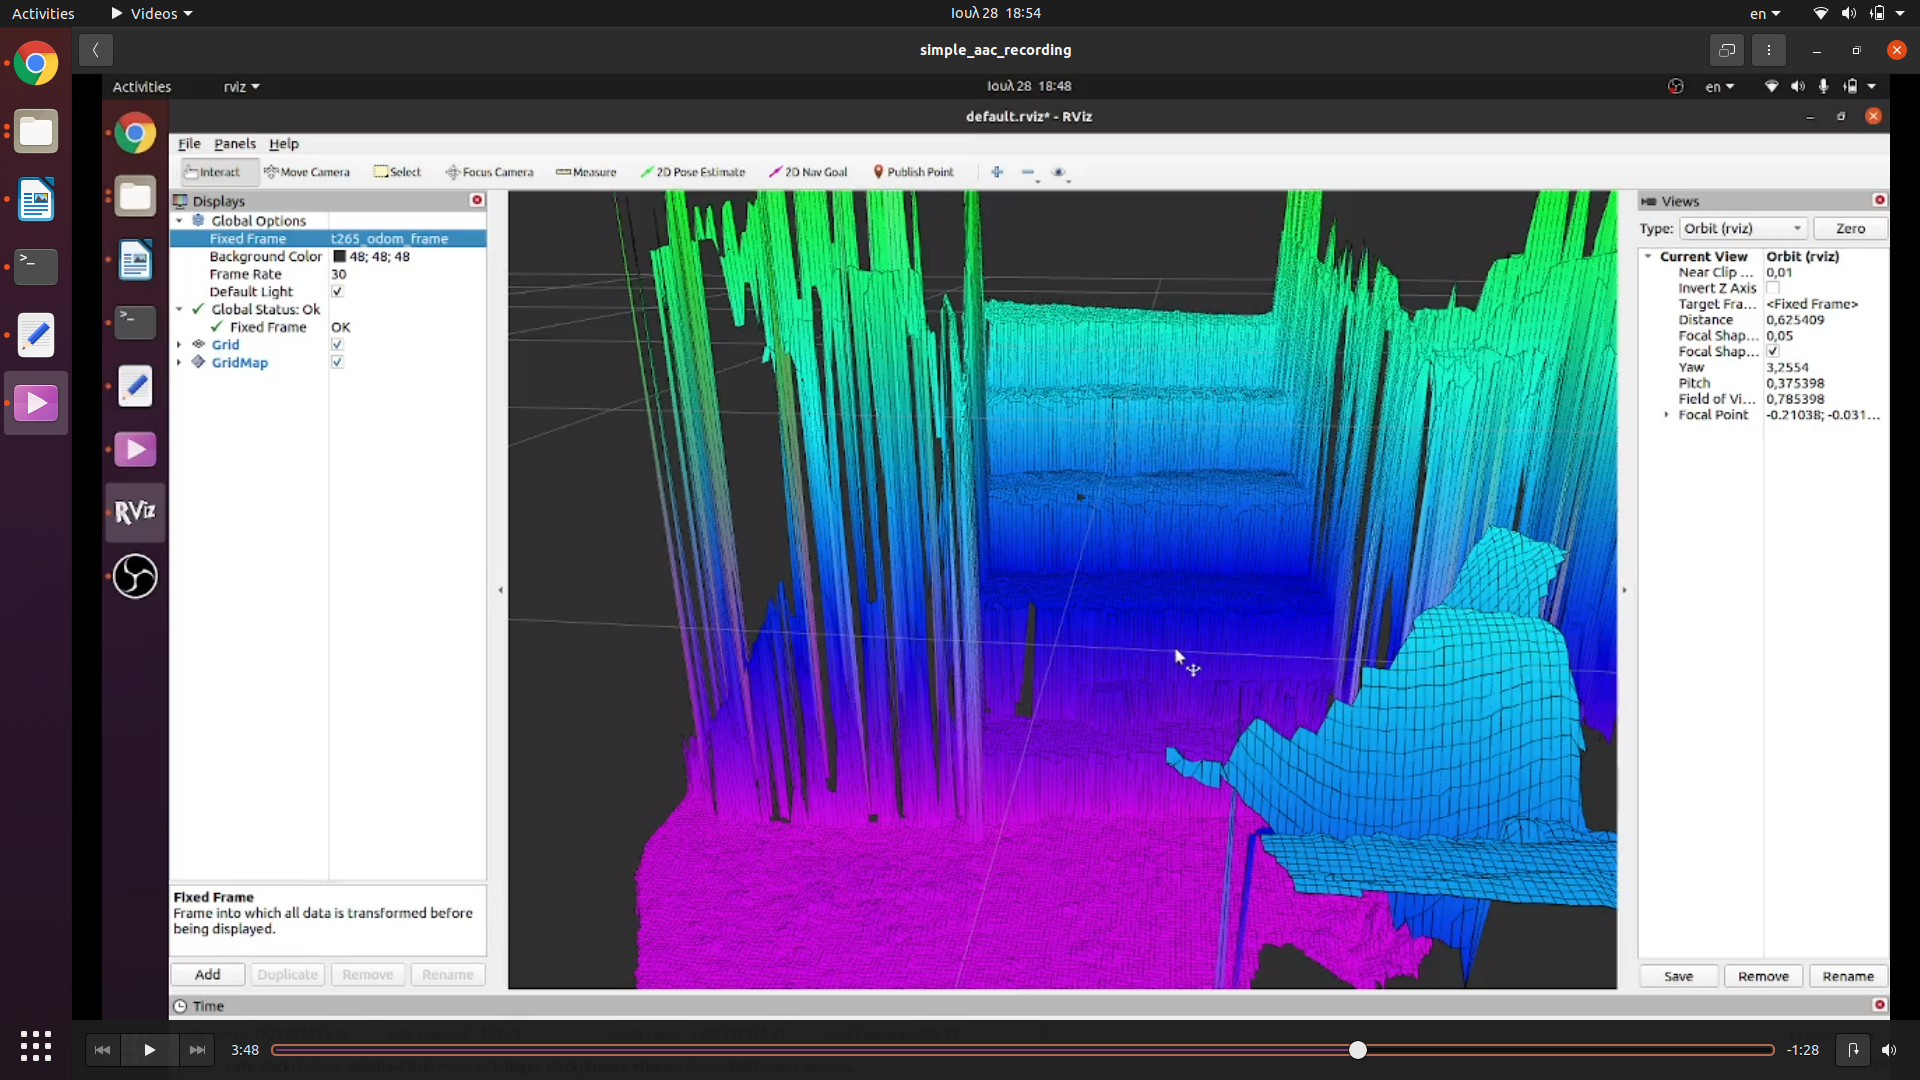
\includegraphics[width=\textwidth,height=\textheight,keepaspectratio]{report1-img017.png} %
	\caption{The chromatic elevation map of the wooden staircase as displayed in Rviz. }
\end{figure}

During the experiment of mapping the wooden staircase, it became evident that this package produces a robot-centric map. That means that in order to tackle the accumulation of uncertainty due to the proprioceptive localization but also to save computational resources (mainly memory) the map is constructed within a finite spherical space around the robot – in our case, the two cameras -. Everything outside this area will not be mapped and if the robot moves, then the spherical space moves with it, thus everything that was previously mapped but is now outside of the spherical area will be forgotten. That means that if we map the staircase but then move about three meters away from it, the stair will vanish from the map and would need to be remapped again if it was desired.

Testing the precision of this method in the same way rtabmap was tested, it is evident that this method has a similar performance. The height of each stair step was measured as registered in the map made with Anybotics Elevation Mapping and was then compared to the real height of the stair steps which is 20cm. Subtracting the measured value from the real value gives us the measurement error. We then plot the absolute value of this error for the first seven stair steps.

With an average error of about 4.1\% the result is comparable to that of rtabmap. This is expected, as the accuracy of the volumetric measurements of objects is primarily affected by the camera's depth accuracy and not the software used to perform SLAM.

\begin{figure}[h] % [h] forces the figure to be output where it is defined in the code (it suppresses floating)
    \centering
    \textbf{Anybotics Elevation Mapping Volumetric Error}\par\medskip
	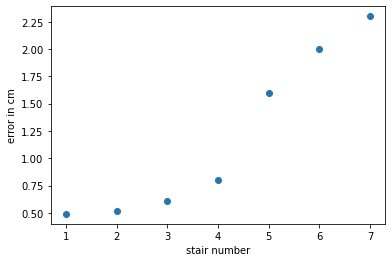
\includegraphics[width=\textwidth,height=\textheight,keepaspectratio]{report1-img018.png} %
	\caption{Absolute error value of stair height in centimeters for the first seven stair steps. }
\end{figure}

Instead of just a pointcloud, this package also produces a gridmap along with an elevation scale and thus could need less processing before being used for applications such as climbing a staircase. However, this also poses drawbacks. Essentially, the map constructed with Anybotics Elevation Mapping is not a 3D map of the environment, but rather a 2.5D map(two-and-a-half dimensional, alternatively pseudo-3D or three-quarter): For every point in the plane on which the robot moves, the elevation of this point is saved the result is plotted in 3D space. This simplifies the data but also creates problems with modelling multiple surfaces that are stacked along the z-axis. For example, if an object is placed 2 meters over a specific stair of the staircase, then the software will assume that the elevation at that specific area is equal to the height at which this object is, while it is important knowledge that there is an obstacle 2 meters over the stair, but the stair itself is not occupied and can be climbed.

To demonstrate the above issue, a floating horizontal platform was placed in front of the turtlebot in the simulated demo. There was enough space under the platform for the simulated robot to get through as can be seen in figure 20. However, in the elevation map, we can see that the floating platform was interpreted as ground elevation and therefore as a high obstacle (figure 21).

It is worth mentioning that the mapping process can also adapt to dynamic environments. Namely, the map remains consistent even if objects inside the mapped environment are being moved during the mapping process. To achieve this, a visibility check is performed based on ray tracing. A visibility map is constructed from the rays connecting the point of the height measurement to the depth sensor’s position at this measurement. This map reflects the maximal height that each cell can have based on the visibility constraint. Namely, if a cell is registered as being high enough to block the sensor's visibility, but the visibility is not being blocked, then that cell violates the visibility constraint and is removed.
As this visibility check is computationally intensive, it is only performed at a lower rate (e.g., 1 Hz).

\begin{figure}[h] % [h] forces the figure to be output where it is defined in the code (it suppresses floating)
    \centering
	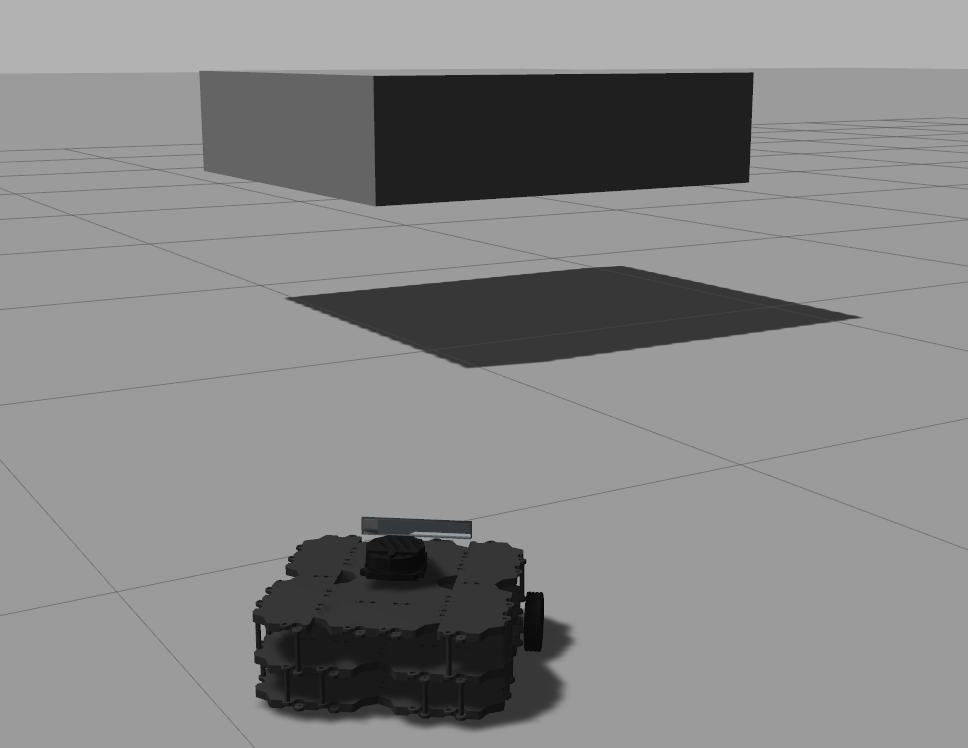
\includegraphics[width=\textwidth,height=\textheight,keepaspectratio]{report1-img024.png} %
	\caption{The floating horizontal platform in Gazebo. }
\end{figure}

\begin{figure}[h] % [h] forces the figure to be output where it is defined in the code (it suppresses floating)
    \centering
	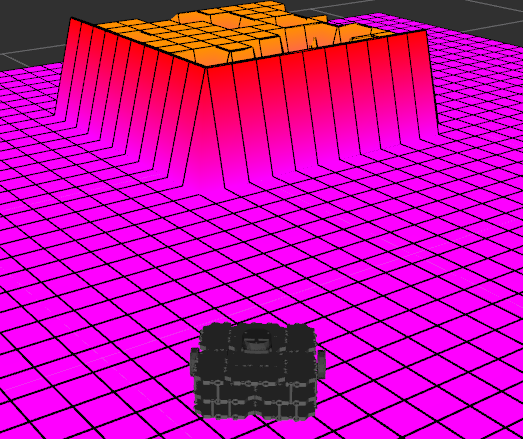
\includegraphics[width=\textwidth,height=\textheight,keepaspectratio]{report1-img025.png} %
	\caption{The elevation map produced with Anybotics Elevation Mapping. }
\end{figure}

\clearpage

\subsubsection{Gradslam}

Gradslam is a fully differentiable dense SLAM framework. Lately, gradient-based learning approaches have had limited success in the context of SLAM, primarily since many of the elements in the standard SLAM pipeline are not differentiable. It is important for a framework to be fully differentiable because each of its components can then be fed into gradient based learning models. For example, a pointcloud in itself is a non-differentiable function. However, producing a meshgrid out of the pointcloud and filtering the grid with a smoothing filter yields a continuous surface which could be descrived as a differentiable function. Processes such as graphics and physics are being made differentiable to embed stronger domain specific information into deep learning algorithms. This has not been the case for SLAM. \href{https://arxiv.org/pdf/1910.10672.pdf}{[22]}

Gradslam provides a repository of differentiable building blocks for a dense SLAM system. One can use these blocks to construct SLAM systems that allow gradients to flow all the way from the outputs of the system (map, trajectory) to the inputs (raw color/depth images, parameters, calibration, etc.). Thus, the error signals indicating task performance could be backpropagated all the way through the SLAM system, to the raw sensor observations.

Namely, similarily to how a simple method like gradient descend is used for estimating a person's height h when given his weight w, by training on a dataset d and minimizing a cost function f, the formal goal of gradslam is to have an expression that relates sensor measurements s to a 3D map m of the environment. From there, given a dataset with a set of sensor measurements S and a set of maps M, we can train a predictor P which given sensor measurements s yields an accurate map m, by minimizing a differentiable cost function F. More formally, the goal is to develop a differentiable mapping function $$ M = GSLAM(s)$$ Then the gradient of that mapping $$\nabla sM$$ can intuitively show that perturbing the sensor measurement s by an infinitesimal ds causes the map M to change by $$\nabla sGSLAM(s)ds$$

\bigskip

The framework consists of a differentiable nonlinear least squares solver, a Differentiable mapping function, a Differentiable map fusion algorithm and a Differentiable ray backprojection algorithm. 

The latest version of pytorch was installed, as it is a prerequisite for running Gradslam. Consequently, Gradslam was installed from source and imported into a python code script to be tested.\href{https://gradslam.readthedocs.io/en/latest/tutorials/tutorial_prerequisits.html}{[23]}

\bigskip
\textit{Testing with our cameras}
\bigskip

The pyrealsense2 library was used to configure and launch the two cameras. Initially, the D435i camera was launched with the purpose of capturing a sequence of RGB-D images (colored images along with their corresponding depth image). Then, the ICL dataset format was used in order to form a gradslam-compatible dataset with the captured images. 

The script initializes RGBDdimages (a class imported from gradslam) using the newly formed dataset and then plots the result. Next, the vertex maps and the normal maps of the staircase dataset were computed and plotted successfully. Those maps are a mathematical representation of our 3D space and in contrast to normal pointclouds they are fully differentiable.

\begin{figure}[h] % [h] forces the figure to be output where it is defined in the code (it suppresses floating)
    \centering
	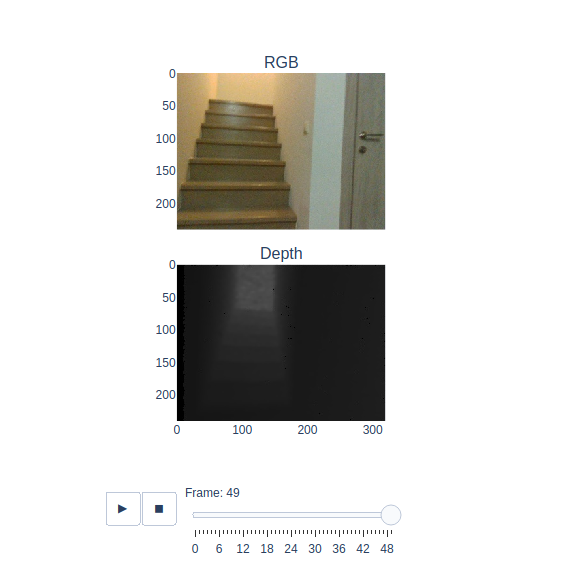
\includegraphics[width=\textwidth,height=\textheight,keepaspectratio]{report1-img019.png} %
	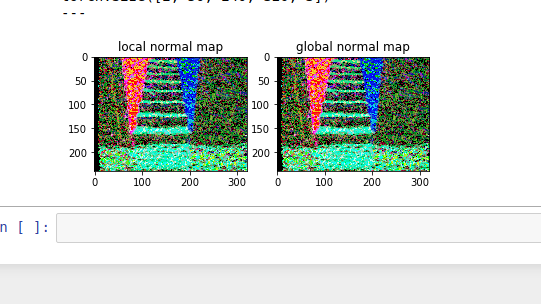
\includegraphics[width=\textwidth,height=\textheight,keepaspectratio,trim={0 4cm 0 1cm},clip]{report1-img020.png} %
	\caption{RGBDimages and vertex maps visualised. }
\end{figure}

\clearpage

Capturing pose data with the T265 camera and incorporating them into the new dataset was the next step. After formatting the data to be compatible with the ICL dataset’s format, the dataset was aggregated to achieve full SLAM. We also tested the provided step-by-step functionality to achieve real-time SLAM. The performance of the package was however notably slower than the performance of the packages tested before, with the map being updated at a frequency of less than 1Hz. 

The final output is comparable to what has been discussed so far. Note, that the aggregation of the dataset with poses received from the T265 camera, did not change the quality of the exported pointclouds at all, even when tested multiple times. We can infer that without modifications of the code provided, gradslam does not make use of the provided pose data at all. Instead, it performs visual-only SLAM (V-SLAM), which means that the algorithm estimates the trajectory that the camera followed by solely reviewing the RGB-D images from the D435i camera.

\begin{figure}[h] % [h] forces the figure to be output where it is defined in the code (it suppresses floating)
    \centering
	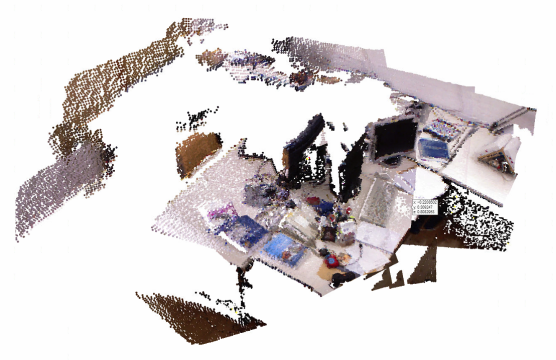
\includegraphics[width=\textwidth,height=\textheight,keepaspectratio]{report1-img021.png} %
	\caption{Pointcloud made with Gradslam on the original ICL dataset. }
\end{figure}

\subsection{Portability}

All of the above experiments were conducted by moving the cameras by hand while having them connected to a main PC via cable. This poses a lot of constraints on the movement and the available viewing angles of the cameras. It also does not reflect the final intended use of the cameras, which is mounting them on a moving quadruped robot. 

This is to be solved by using an NVIDIA Jetson Nano module which is powered by a power bank which outputs 5V – 3A continuous current. The power was delivered via the micro USB port of the Jetson Nano. Alternatively, the on board DC barrel jack can be used.

\begin{figure}[h] % [h] forces the figure to be output where it is defined in the code (it suppresses floating)
    \centering
	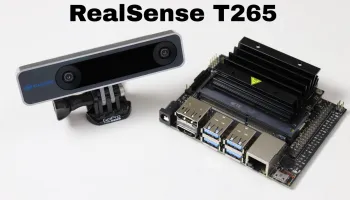
\includegraphics[width=\textwidth,height=\textheight,keepaspectratio]{report1-img022.png} %
	\caption{The realsense T265 camera alongside the Jetson Nano. }
\end{figure}


Rtabmap and Anybotics Elevation Mapping was installed on the Jetson Nano module. Note that it is preferable to use ros-melodic and Ubuntu 18.04 on the Jetson, because otherwise modifications to the linux kernel are required for the software to run. Even so, some dependencies and libraries had to be installed manually and some of them needed to be installed in older versions to work with the Jetson Nano. \href{https://github.com/JetsonHacksNano/installROS}{[24]}

Finally, the installed packages were tested. The results were pretty similar to those conducted on the main laptop. However, in many cases the Jetson module suddenly powered off during the experiments. In some other cases, the software would crash unexpectedly and the module would power off seconds or minutes later. The most prominent explanation is that the power supply via the micro USB port is insufficient. Various users recommend using a DC barrel jack adapter to power the Jetson Nano module. This will soon be tested. \href{https://desertbot.io/blog/jetson-nano-power-supply-barrel-vs-micro-usb}{[25]}

\newpage
[1]	“Tracking camera T265,” Intel® RealSenseTM Depth and Tracking Cameras. https://www.intelrealsense.com/tracking-camera-t265/ .
\bigskip

[2]	“Depth Camera D435i,” Intel® RealSenseTM Depth and Tracking Cameras. https://www.intelrealsense.com/depth-camera-d435i/ .
\bigskip

[3]	“Beginner’s guide to depth (Updated),” Intel® RealSenseTM Depth and Tracking Cameras, Jul. 16, 2019. https://www.intelrealsense.com/beginners-guide-to-depth/ .
\bigskip

[4]	“Simultaneous localization and mapping,” Wikipedia. Jan. 22, 2022. Available:

https://en.wikipedia.org/w/index.php?title=

Simultaneous\_localization\_and\_mapping\&oldid=1067173695
\bigskip

[5]	“Lidar,” Wikipedia. Jan. 30, 2022. Available:

https://en.wikipedia.org/w/index.php?title=Lidar\&oldid=1068915816
\bigskip

[6]	“Differences between the Lidar Systems and Depth Camera – LiDAR and RADAR Information.” https://lidarradar.com/info/differences-between-the-lidar-systems-and-depth-camera.
\bigskip

[7]	R. Horaud, M. Hansard, G. Evangelidis, and C. Menier, An Overview of Depth Cameras and Range Scanners Based on Time-of-Flight Technologies. 2020.
\bigskip

[8]	“Why LiDAR is Doomed.” https://www.voltequity.com/article/why-lidar-is-doomed.
\bigskip

[9]	“Correspondence problem,” Wikipedia. Dec. 29, 2021. Available:

https://en.wikipedia.org/w/index.php?title=Correspondence\_problem\&oldid=1062632962
\bigskip

[10]	“Lidar cameras, Stereo Depth cameras, Coded light and Tracking cameras from Intel RealSense,” Intel® RealSenseTM Depth and Tracking Cameras. https://www.intelrealsense.com/ .
\bigskip

[11]	Pysource, Distance detection with Depth Camera (Intel Realsense d435i) - Opencv with Python tutorial, (2021). 

Available: https://www.youtube.com/watch?v=mFLZkdH1yLE
\bigskip

[12]	“GitHub - IntelRealSense/realsense-ros: Intel(R) RealSense(TM) 

ROS Wrapper for D400 series, SR300 Camera and T265 Tracking Module.”

https://github.com/IntelRealSense/realsense-ros 
\bigskip

[13]	“Surveying the Stars | Astronomy.”

https://courses.lumenlearning.com/astronomy/chapter/surveying-the-stars/ .
\bigskip

[14]	“Intel® MovidiusTM Vision Processing Units (VPUs),” 

Intel. https://www.intel.com/content/www/us/en/products/details/processors/movidius-vpu.html .
\bigskip

[15]	“USB 2 for T265,” Intel RealSense Help Center. http://support.intelrealsense.com/hc/en-us/community/posts/360038384494-USB-2-for-T265 .
\bigskip

[16]	“navigation/ROS\_Wrappers - ROS Wiki.” http://wiki.ros.org/navigation/ROS\_Wrappers .
\bigskip

[17]	“T265 Device not detected,” Intel RealSense Help Center.

http://support.intelrealsense.com/hc/en-us/community/posts/360033359193-T265-Device-not-detected .
\bigskip

[18]	“RTAB-Map,” RTAB-Map. http://introlab.github.io/rtabmap/ .
\bigskip

[19]	matlabbe, RTAB-Map for iOS - LiDAR Scanner App. Available:

https://www.youtube.com/watch?v=rVpIcrgD5c0
\bigskip

[20]	“ANYbotics/elevation\_mapping,” Dec. 19, 2020.

https://github.com/ANYbotics/elevation\_mapping .
\bigskip

[21]	P. Fankhauser, M. Bloesch, and M. Hutter, “Probabilistic Terrain Mapping for Mobile Robots With Uncertain Localization,” IEEE Robot. Autom. Lett., vol. 3, no. 4, pp. 3019–3026, Oct. 2018, doi: 10.1109/LRA.2018.2849506.
\bigskip

[22]	K. M. Jatavallabhula, S. Saryazdi, G. Iyer, and L. Paull, “gradSLAM: Automagically differentiable SLAM,” ArXiv191010672 Cs, Nov. 2020, Available: http://arxiv.org/abs/1910.10672
\bigskip

[23]	“Prerequisits — gradslam 0.1.0 documentation.”

https://gradslam.readthedocs.io/en/latest/tutorials/tutorial\_prerequisits.html .
\bigskip

[24]	JetsonHacksNano, installROS. 2022. Available: 

https://github.com/JetsonHacksNano/installROS
\bigskip

[25]	“Jetson Nano Power Supply (Barrel vs. Micro USB) | desertbot.io.” https://desertbot.io/blog/jetson-nano-power-supply-barrel-vs-micro-usb .
\bigskip


\end{document}
